\section{The British electricity spot market: Wolfram (1999)}\label{sec:03-electricity}

The sugar study of \cref{sec:03-sugar} validated the conduct-parameter method with historical cost data.
\citet{Wolfram1999} performs a second validation in a modern market where marginal cost is close to observable.
Electricity generation suits the exercise. Short-run marginal cost is almost entirely the cost of fuel, and fuel cost
depends only on the fuel price and on how efficiently a plant converts fuel into electricity. After the British
industry was privatized in 1990, two firms owned most fossil-fuel generation in England and Wales, and demand was
extremely inelastic. Standard oligopoly models therefore predicted very high markups. Wolfram measures markups
directly, compares them with these predictions, and checks them against two methods that ignore cost data. The
section ends with the studies of restructured US and Spanish markets that built on her design
(\cref{sec:03-wolfram-later}).

\subsection{The question and the institutions}\label{sec:03-wolfram-setting}

\casehead{The question}
How much market power did the two dominant generators exercise in the British electricity spot market, and do
standard oligopoly models predict their prices? A second question is methodological. Do approaches that treat
marginal cost as unobserved recover the markups that cost data reveal? The answers matter beyond Britain. The British
reform was one of the first attempts to build a fully competitive market for electricity generation, and the United
States and other countries were preparing similar reforms \citep[p.~805]{Wolfram1999}. Cournot and supply function
models were the standard tools for predicting market power in such markets
\citep{GreenNewbery1992,BorensteinBushnell1999}.

\casehead{Why electricity}
Several features make electricity markets prone to market power and well suited to measuring it
\citep[pp.~687--688]{KelloggReguant2021}. Electricity is a homogeneous good, but plants with very different technologies
and costs produce it at the same time. It has been extremely difficult to store economically, and demand is quite
inelastic in the short and medium run. Together these features create large price fluctuations and moments of
scarcity in which market power can be substantial. Supply must match demand second by second over a shared grid, so a
central authority coordinates dispatch. The data are unusually granular, and plausible shifters of both supply and
demand are observed.

Britain's reform was followed by restructuring in many countries. In the United States the process was partial and
slow. It began in California, New England and the Pennsylvania-New Jersey-Maryland market (PJM). Restructuring
elsewhere was put on hold after the California crisis of 2000 and 2001, and large areas still regulate generation on
a cost-of-service basis \citep[p.~688]{KelloggReguant2021}. \citet{Cicala2020} measures what the move to markets
achieved. He exploits the staggered entry of US power control areas into market-based dispatch between 1999 and 2012. A
\emph{power control area} is a region of the grid in which a single operator balances supply and demand.
His data cover hourly demand, the hourly output of most plants and engineering estimates of their costs. For each
hour he compares actual generation cost with the least cost of producing the same quantity, which is the merit-order
calculation of \cref{sec:03-wolfram-data}. A difference-in-differences comparison finds that joining a market raised
the gains from trade between areas by 55 percent. It cut departures from the least-cost merit order within an area by
16 percent \citep[p.~689]{KelloggReguant2021}.

\casehead{Industry structure}
Before April 1990 a single state body, the Central Electricity Generating Board (CEGB), owned and operated the
generating plants and the transmission grid. It sold to twelve government-owned Area Boards, which distributed
electricity in England and Wales. At privatization the Area Boards became twelve Regional Electricity Companies
(RECs), distributors with local franchises and price-capped distribution charges. Transmission went to the National
Grid Company. The CEGB's plants were split three ways. Nuclear Electric received the twelve nuclear stations, with
about 9 gigawatts (GW) of capacity, and stayed in the public sector for six years. National Power received 52 percent
of the CEGB's capacity (roughly 30 GW) and PowerGen 33 percent (roughly 20 GW). Interconnectors with Scotland and
France and two pumped-storage stations supplied several more gigawatts. Between March 1990 and the end of 1994 about
7 GW of new capacity entered, more than half of it owned by firms other than National Power and PowerGen
\citep[pp.~806--807]{Wolfram1999}.

\casehead{The Pool}
All wholesale trade passed through a central market, the \emph{Pool}, which worked financially as a day-ahead spot
market. Each day is divided into 48 half-hour periods, with one price per period. Every day each generator submits a
bid schedule stating the prices at which it will supply power from each of its generating units on the following day.
The Pool administrator ranks the bids and, using its demand forecast, finds for each half-hour the bid of the most
expensive unit needed to meet demand. That bid is the \emph{system marginal price} (SMP). The \emph{pool price} adds a
capacity payment to the SMP, and a charge called uplift is added after demand is realized to cover forecast errors and
ancillary services \citep[p.~807 and n.~7]{Wolfram1999}.

\casehead{Contracts}
Most trade was hedged by financial contracts between generators and their customers. A \emph{two-way contract}, or
\emph{contract for differences}, fixes a strike price for a contracted volume. The generator pays the customer the
excess of the pool price over the strike price and receives the shortfall when the pool price is lower. A
\emph{one-way contract} protects only the customer, who never pays more than the strike price. At privatization the
government set up initial contracts between the RECs and the generators that ran from one to three years. In the first
year they covered 85 to 90 percent of the capacity of National Power and PowerGen. By fiscal year 1993 cover had fallen
to just above 70 percent. All initial contracts expired at the end of March 1993, and their replacements covered only
about half of the generators' capacity \citep[p.~808]{Wolfram1999}. Little information on the terms of the contracts is
public (n.~8).

\casehead{Regulatory oversight}
Pool prices were not regulated directly. The industry regulator, who headed the Office of Electricity Regulation
(OFFER), held a blunt instrument. He could refer the generators to the Monopolies and Mergers Commission (MMC), which
could break up National Power and PowerGen. By the end of 1994 OFFER had issued four statements on pool prices. The
first three recommended minor institutional changes but expressed concern about price levels and market power. In the
fourth, in February 1994, the regulator offered a deal. He would not refer the generators if they sold 10 to 15 percent
of their plant to potential competitors and accepted a price cap from April 1, 1994 \citep[p.~808]{Wolfram1999}. The cap
applied to the
time-weighted average pool price over the fiscal year, with a higher cap on the demand-weighted average
\citep[p.~818]{Wolfram1999}.

\casehead{Why theory predicts high markups}
Short-run electricity demand is very inelastic. Static oligopoly theory then predicts markups so large that an interior
equilibrium may fail to exist.

\begin{proposition}[Inelastic demand and Cournot equilibrium]\label{prop:03-no-interior-cournot}
Let firms compete in quantities with marginal costs $MC_i > 0$, and let market demand have constant elasticity
$\varepsilon > 0$. In any interior Cournot equilibrium,
\begin{enumerate}[label=(\roman*)]
\item Each firm's Lerner index is $L_i = \frac{s_i}{\varepsilon}$.
\item Every active firm has a share $s_i < \varepsilon$.
\item With $N$ symmetric firms, an interior equilibrium requires $N > \frac{1}{\varepsilon}$.
\end{enumerate}
\end{proposition}

\begin{proof}
Firm $i$'s first-order condition is $P + q_i P'(Q) = MC_i$. Dividing by $P$ and using $-\frac{Q P'}{P} =
\frac{1}{\varepsilon}$ gives
\begin{equation*}
\frac{P - MC_i}{P} = -\frac{q_i P'(Q)}{P} = \frac{q_i}{Q}\cdot\frac{1}{\varepsilon} = \frac{s_i}{\varepsilon},
\end{equation*}
which is (i). Since $MC_i > 0$, the Lerner index is below one, so $s_i < \varepsilon$, which is (ii). With symmetric
firms $s_i = \frac{1}{N}$, and (ii) becomes $N > \frac{1}{\varepsilon}$.
\end{proof}

Part (ii) restates \cref{rem:02-inelastic}. The proposition has a stark implication for Britain. With a constant
elasticity of 0.17, the value at the sample means used below, an interior Cournot equilibrium needs at least six
symmetric firms. With two firms of equal size the formula gives
$L_i = \frac{0.5}{0.17} = 2.9$, an impossible markup. Each firm's perceived marginal revenue
$P(1 - \frac{s_i}{\varepsilon})$ is negative, so cutting output raises revenue and lowers cost. Firms keep withholding
output until something else binds. Demand may become more elastic at high prices, as it does on a linear demand curve.
The regulator may step in, or forward contracts may reduce each firm's gain from a higher spot price
(\cref{prop:03-contracts}). An upper capacity limit cannot stop the withdrawal, because it does not restrict a
reduction in output. Panel (a) of \cref{fig:03-merit-order} shows why
withholding is so profitable here. The industry marginal cost curve is flat over a wide range and then nearly
vertical. Demand is nearly vertical too. A small reduction in the quantity offered moves the market onto the steep
segment and multiplies the price.

\begin{figure}[tbp]
\centering
\begin{subfigure}[b]{0.48\textwidth}
\centering
\begin{tikzpicture}[scale=0.92,>=Stealth]
\draw[->] (0,0) -- (5.6,0) node[below] {\small $Q$};
\draw[->] (0,0) -- (0,5.3) node[left] {\small $P$};
\draw[thick,name path=mc] (0,0.3) -- (1.0,0.3) -- (1.0,1.2) -- (4.2,1.45) -- (4.2,2.0) -- (4.5,2.0) -- (4.65,2.6)
  -- (4.75,3.4) -- (4.8,4.6);
\draw[thick,dashed,name path=sw] (3.3,1.45) -- (3.3,2.0) -- (3.6,2.0) -- (3.75,2.6) -- (3.85,3.4) -- (3.9,4.6);
\draw[thick,gray,name path=dem] (4.05,0) -- (3.75,4.6);
\path[name intersections={of=mc and dem,by=Ec}];
\path[name intersections={of=sw and dem,by=Ew}];
\fill (Ec) circle (1.6pt);
\fill (Ew) circle (1.6pt);
\draw[dotted] (Ec) -- (Ec -| 0,0) node[left] {\small $P^{c}$};
\draw[dotted] (Ew) -- (Ew -| 0,0) node[left] {\small $P^{w}$};
\node[right,font=\footnotesize] at (4.8,4.3) {$MC(Q)$};
\node[left,font=\footnotesize] at (3.72,4.3) {$S^{w}$};
\node[gray,font=\footnotesize,anchor=west] at (4.05,0.25) {$D$};
\draw[<->] (3.9,4.8) -- (4.8,4.8);
\node[font=\footnotesize,anchor=south] at (4.35,4.8) {$\Delta$};
\node[font=\footnotesize] at (1.9,0.7) {nuclear};
\node[font=\footnotesize] at (2.2,1.65) {coal};
\end{tikzpicture}
\caption{Merit order and withholding}
\end{subfigure}
\hfill
\begin{subfigure}[b]{0.48\textwidth}
\centering
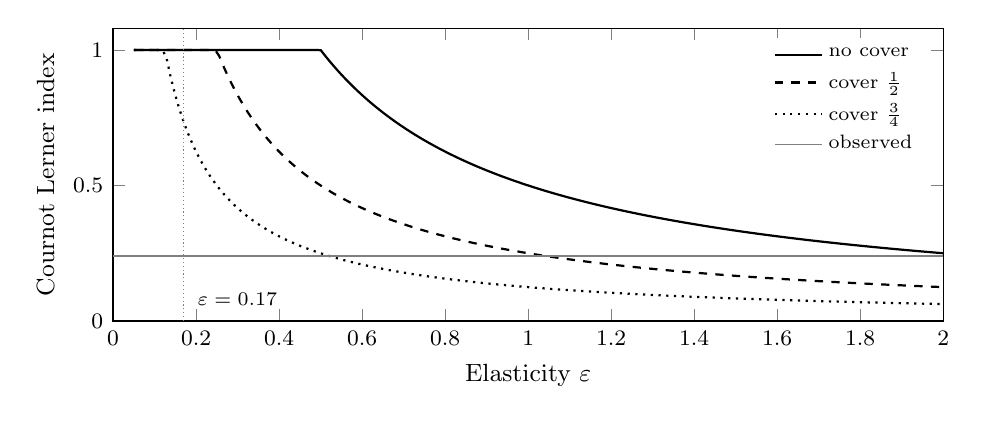
\begin{tikzpicture}
\begin{axis}[width=\linewidth, height=5.3cm, xmin=0, xmax=2, ymin=0, ymax=1.08,
  xlabel={\small Elasticity $\varepsilon$}, ylabel={\small Cournot Lerner index},
  tick label style={font=\footnotesize},
  legend style={font=\scriptsize, draw=none, fill=white, at={(0.98,0.97)}, anchor=north east},
  legend cell align=left]
\addplot[thick, domain=0.05:2, samples=200] {min(1, 0.5/x)};
\addlegendentry{no cover}
\addplot[thick, dashed, domain=0.05:2, samples=200] {min(1, 0.25/x)};
\addlegendentry{cover $\frac{1}{2}$}
\addplot[thick, dotted, domain=0.05:2, samples=200] {min(1, 0.125/x)};
\addlegendentry{cover $\frac{3}{4}$}
\addplot[gray, domain=0:2] {0.24};
\addlegendentry{observed}
\draw[gray, densely dotted] (axis cs:0.17,0) -- (axis cs:0.17,1.08);
\node[font=\scriptsize, anchor=west] at (axis cs:0.18,0.08) {$\varepsilon = 0.17$};
\end{axis}
\end{tikzpicture}
\caption{Cournot markups and contract cover}
\end{subfigure}
\caption{Why oligopoly theory predicts high electricity markups. Panel (a) is a schematic. The industry marginal cost
curve $MC(Q)$ ranks plants from cheapest to most expensive. Demand $D$ is nearly vertical, so withholding a quantity
$\Delta$ of low-cost capacity shifts the offered supply to $S^{w}$ and raises the price from $P^{c}$ to $P^{w}$. Panel
(b) plots the Cournot Lerner index $\min\{1, \frac{s_i}{\varepsilon}(1 - \frac{x_i}{q_i})\}$ of a firm with share
$s_i = \frac{1}{2}$ and contract cover $\frac{x_i}{q_i}$, from \eqref{eq:03-contracts}. Under constant-elasticity
demand, the value one marks the region with no interior equilibrium. The gray horizontal line is the observed average Lerner index of 0.24.}
\label{fig:03-merit-order}
\end{figure}

\subsection{Data and the measurement of marginal cost}\label{sec:03-wolfram-data}

\casehead{The data}
The sample covers 25,639 half-hour periods: nearly every half-hour of six months (January, February, March, April,
July and November) in each of 1992, 1993 and 1994, 18 months in all. About 40 periods are missing. The Pool data come
from the National Grid Company, which lacked some variables before 1992 \citep[pp.~810, 822 and n.~49]{Wolfram1999}.
Price is the SMP, which excludes the capacity payment, because the cost measure covers only fuel. Quantity is the
energy metered in each half-hour, including transmission losses. Appendix Table A1 of the paper reports a mean SMP of
\pounds 22.26 per megawatt-hour (MWh), with a standard deviation of 7.10. The pool selling price, which adds the
capacity payment and uplift, has a mean of \pounds 24.40 and a standard deviation of 10.17. Mean quantity is 16,211
MWh per half-hour, with a standard deviation of 2,839. Energy of 16,211 MWh delivered in half an hour is an average
rate of about 32 GW.

\casehead{Plant marginal cost}
The short-run marginal cost of a fossil-fuel plant is the cost of the fuel it burns per unit of electricity. Let plant
$k$ burn fuel with price $w_k$ in pounds per gigajoule (GJ) and convert fuel energy into electricity with
\emph{thermal efficiency} $e_k \in (0, 1)$. One MWh equals 3.6 GJ, so the plant needs $\frac{3.6}{e_k}$ GJ of fuel per
MWh, a quantity called its \emph{heat rate} $h_k$. Its marginal cost is
\begin{equation}\label{eq:03-plant-mc}
mc_k = w_k\, h_k = \frac{3.6\, w_k}{e_k} \quad \text{(pounds per MWh)}.
\end{equation}
For illustration, take coal at \pounds 1.50 per GJ plus \pounds 0.08 of transport and a hypothetical coal plant with an
efficiency of 36 percent. Then $mc_k = \frac{3.6 \times 1.58}{0.36} = 15.8$, inside the range of the flat coal segment of
\cref{fig:03-wolfram-scatter}.

Each input of \eqref{eq:03-plant-mc} is measured with unusual precision \citep[p.~810]{Wolfram1999}. Before
privatization, the \emph{CEGB Statistical Yearbook} published the thermal efficiency of every coal, oil and gas plant.
\citet{GreenNewbery1992} distilled 20 years of these figures into efficiencies under optimal operating conditions, and
Wolfram replaces them with later engineering estimates where plants had been upgraded. Such data later became
competitively sensitive. They are available only because the industry had recently been public. New combined-cycle gas
turbine (CCGT) plants are assumed to have an efficiency of 45 percent. Fuel prices for oil, gas peaking and CCGT plants
are market prices. Coal was bought from British Coal under contracts. The first contracts, which expired in March 1993,
were effectively take-or-pay and supplied more coal than the generators burned. To capture the replacement cost of coal,
Wolfram uses the prices of the next two contracts. Coal burned before the end of March 1994 is valued at 150 pence per
GJ, and coal burned afterwards at 137 pence. Transport costs average 8 pence per GJ, about 5 percent of fuel costs. Nuclear stations are
assigned \pounds 13 (Magnox, the first-generation gas-cooled reactors) and \pounds 11 (advanced gas-cooled reactors)
per MWh. These figures are too high, but
nuclear plants are never marginal. Pumped storage is costed at the average pool price during pumping, adjusted for
efficiency, and imports from Scotland and France at their bid prices.

\casehead{Capacity and the merit order}
A plant's available capacity varies with maintenance and age. Generators may also withhold capacity strategically to
raise capacity payments \citep{WolakPatrick1997}. Wolfram therefore assigns each plant a capacity equal to the mean
plus one half standard deviation of its declared daily capacity in the month. This is on average 85 percent of the
maximum capacity the plant declared for the year. Weighted by plant size the average is 100 percent. The high-availability case of \cref{tab:03-wolfram-robust}, the mean
plus a full standard deviation, raises the unweighted average to 92 percent \citep[pp.~810--811, 816]{Wolfram1999}.
Sorting plants by marginal cost
gives the industry marginal cost curve, called the \emph{merit order}. Index months by $\mu$, and let month $\mu$ have
plants ordered so that $mc_{(1)} \le mc_{(2)} \le \dots$, with capacities $K_{(1)}, K_{(2)}, \dots$. Then
\begin{equation}\label{eq:03-merit-order}
MC_\mu(Q) = mc_{(j)} \qquad \text{for } \sum_{l < j} K_{(l)} < Q \le \sum_{l \le j} K_{(l)}.
\end{equation}
This nondecreasing step function is the marginal cost of producing $Q$ at least cost. Each half-hour $t$ of month $\mu$
yields a markup $L_t = \frac{P_t - MC_\mu(Q_t)}{P_t}$.

\begin{remark}[What the merit-order cost measures]\label{rem:03-merit-order}
Without firm-level quantities, Wolfram cannot compute each firm's own marginal cost. The merit order supplies an
industry marginal cost directly. Under least-cost dispatch every running plant has $mc_k \le MC_\mu(Q_t)$ and the
marginal plant has exactly $MC_\mu(Q_t)$. If every firm operates a plant at the margin, then $MC_{it} = MC_\mu(Q_t)$ for
all $i$, and
any weights in \cref{prop:03-aggregation} give the same industry marginal cost. If firms withhold low-cost units, the
units that run are more expensive than least-cost dispatch requires. The measured markup then compares price with the
efficient marginal cost, so it also counts the productive inefficiency that withholding creates.
\end{remark}

\casehead{What the data show}
\Cref{fig:03-wolfram-scatter} reproduces the paper's Figure 2 for January and July 1993, a winter and a summer month at
the midpoint of the sample (n.~17). The marginal cost curve rises over the first few gigawatt-hours, where nuclear and
other cheap plants sit. It is then almost flat, between about \pounds 14 and \pounds 17 per MWh, over a wide range where
coal plants are marginal. Near capacity it turns almost vertical, around 26 to 28 GWh per half-hour in January and 21
to 23 GWh in July, when plants are out for summer maintenance. Every observed price lies above marginal cost. In January
prices run from about \pounds 17 to \pounds 35, and the gap widens with quantity. July prices are more dispersed, with a
band near \pounds 31 at low quantities, a cluster around \pounds 50 and one price above \pounds 100. Prices were more
volatile after March 1993, when the initial contracts expired (n.~17). The clouds sit on the flat part of the cost
curve, far from the steep segment where withholding by a duopoly would push them.

\begin{figure}[htbp]
\centering
\begin{subfigure}[b]{0.72\textwidth}
\centering
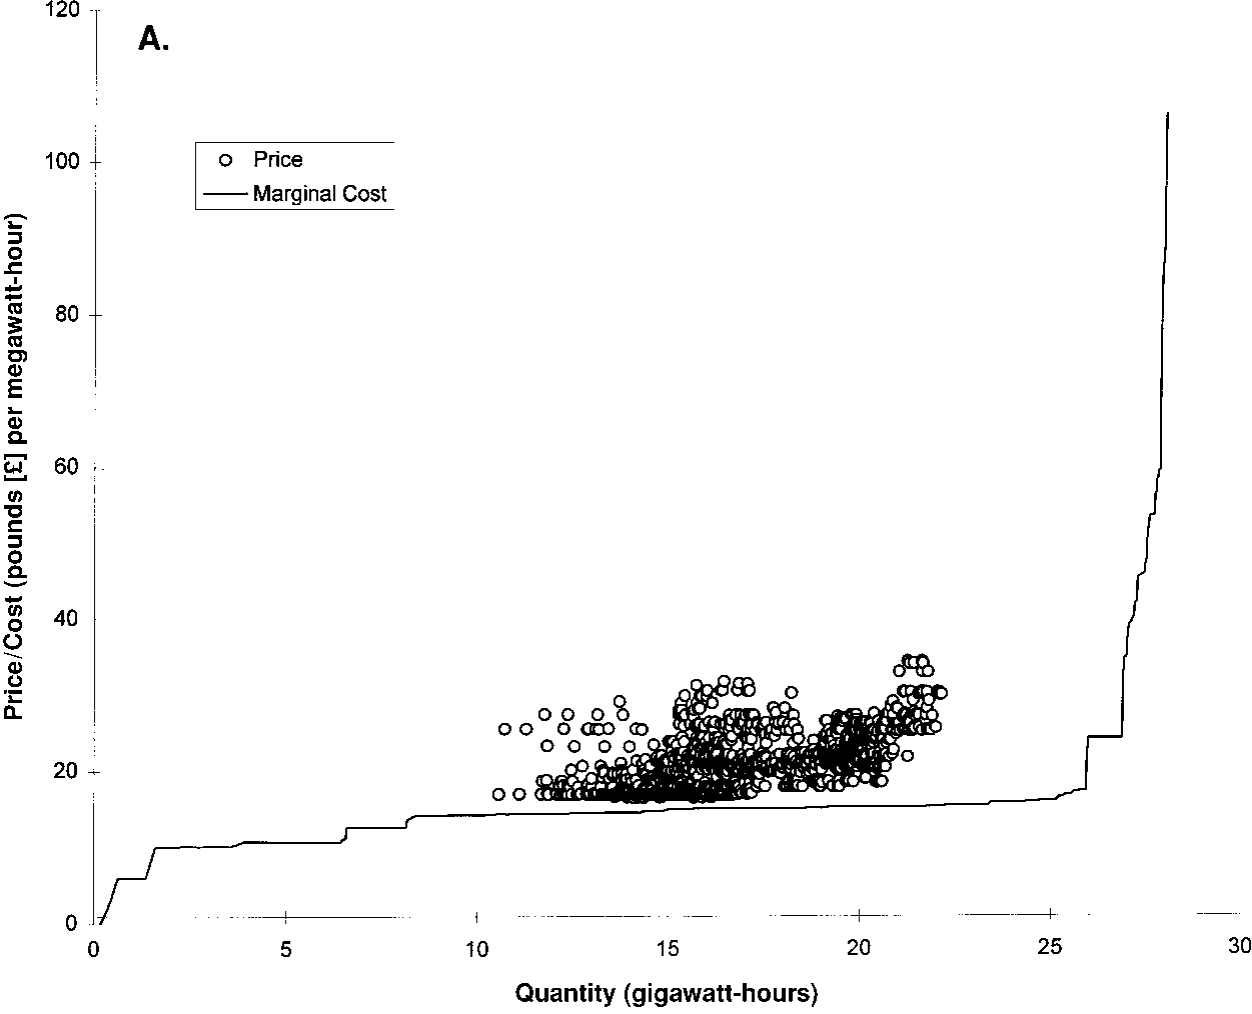
\includegraphics[width=\linewidth]{figures/ch03/wolfram1999_fig2a.png}
\caption{January 1993}
\end{subfigure}

\medskip
\begin{subfigure}[b]{0.72\textwidth}
\centering
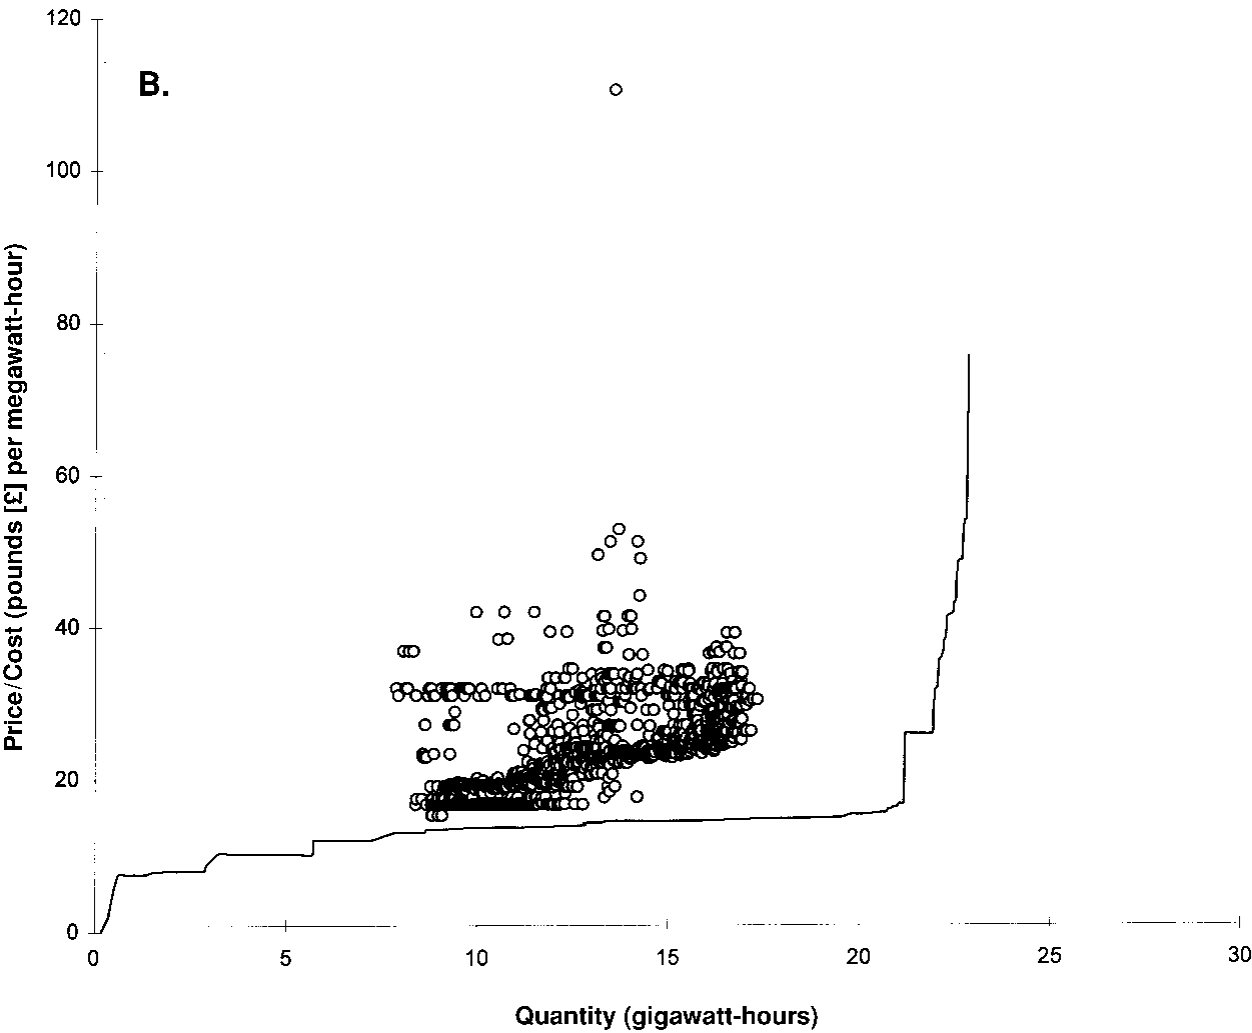
\includegraphics[width=\linewidth]{figures/ch03/wolfram1999_fig2b.png}
\caption{July 1993}
\end{subfigure}
\caption{Pool prices (circles, one per half-hour) and the merit-order marginal cost curve (line), in pounds per MWh
against quantity in gigawatt-hours per half-hour. Source: \citet{Wolfram1999}, Figure 2.}
\label{fig:03-wolfram-scatter}
\end{figure}

\subsection{The model and the direct measure of conduct}\label{sec:03-wolfram-model}

\casehead{Demand, cost and the firm supply relation}
Wolfram's framework is the supply relation of \cref{sec:03-framework} written for half-hours $t$
\citep[pp.~808--809]{Wolfram1999}. Demand is
\begin{equation*}
D_t = D(P_t, X_t, u^d_t),
\end{equation*}
with observed demand shifters $X_t$ such as weather and a demand shock $u^d_t$. Pool demand does respond to price. Some
large users buy directly from the Pool or on contracts tied to pool prices. They switch to backup generators, shut down
energy-intensive processes, or reschedule maintenance when prices are high. Demand also depends on prices in other
half-hours, which the notation suppresses (n.~10). Generator $i$ has marginal cost $MC_{it} = MC_i(q_{it}, Z_{it},
u^s_{it})$, with cost shifters $Z_{it}$ and a cost shock $u^s_{it}$, and profit
\begin{equation*}
\Pi_{it} = P(Q_t, X_t, u^d_t)\, q_{it} - C_i(q_{it}, Z_{it}, u^s_{it}).
\end{equation*}
Its first-order condition, written with a firm-level conduct parameter $\tilde\theta_{it}$, is
\begin{equation}\label{eq:03-wolfram-foc}
P_t = MC_i(q_{it}, Z_{it}, u^s_{it}) - \tilde\theta_{it}\, q_{it}\, P_Q(Q_t, X_t, u^d_t),
\end{equation}
where $P_Q$ is the slope of inverse demand. Cournot conduct is $\tilde\theta_{it} = 1$ and price taking is
$\tilde\theta_{it} = 0$. In the language of \cref{cor:03-benchmarks}, $\tilde\theta_{it} = 1 + r_i$.

\casehead{Aggregation}
Firm-level quantities are not available, so the analysis works with the industry. Applying
\cref{prop:03-aggregation} to \eqref{eq:03-wolfram-foc} with weights $\varphi_{it}$ gives
\begin{equation}\label{eq:03-wolfram-supply}
P_t = MC(Q_t, \mathbf{Z}_t, u^s_t) + \frac{P_t}{\varepsilon_t}\,\theta_t,
\qquad
\theta_t = \sum_{i=1}^{N} \varphi_{it}\,\frac{q_{it}}{Q_t}\,\tilde\theta_{it},
\end{equation}
which is Wolfram's eq.~(5). Rearranging gives her eq.~(6),
\begin{equation}\label{eq:03-wolfram-theta}
\theta_t = \varepsilon_t\,\frac{P_t - MC_t}{P_t}.
\end{equation}
Wolfram writes $\eta$ for the elasticity and $\kappa_{it}$ for the weights. With $\varphi_{it} = \frac{1}{N}$ and a common
$\tilde\theta_t$, industry conduct is $\theta_t = \frac{\tilde\theta_t}{N}$. It equals 1 for joint profit maximization,
$\frac{1}{N}$ for Cournot and 0 for perfect competition. For this reason $\frac{1}{\theta_t}$ is sometimes read as an
``equivalent number of firms.'' Wolfram treats $\theta_t$ as a summary measure, the elasticity-adjusted markup. She makes
no claim about the conjectures that firms hold (n.~12, citing \citealp{Corts1999}).

\begin{remark}[Markups as transfers]\label{rem:03-wolfram-welfare}
With very inelastic demand, even large markups cause little deadweight loss. Approximate demand by a straight line near
the equilibrium and take marginal cost as flat. Pricing at $P$ instead of $MC$ reduces quantity by about
$\varepsilon Q\frac{P - MC}{P}$, so the Harberger triangle is
\begin{equation*}
DWL \approx \frac{1}{2}(P - MC)\,\varepsilon Q\,\frac{P - MC}{P}
\qquad\Longrightarrow\qquad
\frac{DWL}{PQ} \approx \frac{1}{2}\,\varepsilon L^2 = \frac{1}{2}\,\theta L.
\end{equation*}
With $\varepsilon = 0.17$ and $L = 0.24$, the loss is about 0.5 percent of expenditure, while the transfer
$\frac{(P - MC)Q}{PQ} = L$ is 24 percent. This is why Wolfram also reports quantity-weighted average markups, which speak
to the surplus transferred to producers (p.~814).
\end{remark}

\casehead{The demand slope}
Marginal cost is measured, so only the elasticity is missing from \eqref{eq:03-wolfram-theta}. Wolfram does not
estimate it for this purpose. She assumes linear demand with slope $D_p = \frac{\partial D}{\partial P} = -125$, which
makes her numbers comparable with the simulations of \citet{GreenNewbery1992} \citep[p.~811]{Wolfram1999}. The units are
MWh per half-hour per pound per MWh. A fall of 125 MWh within a half-hour is an average rate of 250 megawatts, or
0.25 GW, which is the slope $b = 0.25$ that Green and Newbery report in gigawatts. Their low and high cases correspond to
$D_p = -50$ and $D_p = -250$. With linear demand,
\begin{equation}\label{eq:03-wolfram-theta-linear}
\varepsilon_t = -D_p\,\frac{P_t}{Q_t}
\qquad\Longrightarrow\qquad
\theta_t = \varepsilon_t\,\frac{P_t - MC_t}{P_t} = -D_p\,\frac{P_t - MC_t}{Q_t}.
\end{equation}
At the sample means, $\varepsilon = \frac{125 \times 22.26}{16{,}211} = 0.17$. This is in the range of short-run
elasticities found elsewhere \citep{Taylor1975}. The largest elasticity that \citet{PatrickWolak1997} find for customers
on pool-price contracts is about 0.3, for water companies, a group unusually sensitive to price. With an average Lerner
index of 0.241, \eqref{eq:03-wolfram-theta-linear} at the means gives $\theta = \frac{125 \times 0.241 \times
22.26}{16{,}211} = 0.041$.

Later work confirms that short-run electricity demand is very inelastic. One reason is that many households face
retail prices that do not vary with wholesale conditions \citep[p.~709]{KelloggReguant2021}. \citet{ReissWhite2005}
exploit the tiers of California tariffs in household survey data. They find an average elasticity of $-0.39$, which
reflects medium-run to long-run responses. \citet{Ito2014} compares households on either side of a utility border in
Orange County. He finds an elasticity of about $-0.08$ with respect to the average price. \citet{Shaffer2020} estimates
about $-0.04$ from bunching at a tariff kink in British Columbia \citep[pp.~710--711]{KelloggReguant2021}. These are
retail residential elasticities, and none measures the response of pool demand. Still, they bracket the value of 0.17
assumed here and the rotation estimates of about 0.1 in \cref{sec:03-wolfram-neio}.

\begin{example}[The Cournot benchmark under the assumed demand]\label{ex:03-wolfram-cournot}
Extend the linear demand through the sample means: $Q = 125(\bar\alpha - P)$ with choke price $\bar\alpha = 22.26 +
\frac{16{,}211}{125} = 151.95$. Let a symmetric duopoly have flat marginal cost $c = 16$, roughly the level of the coal
segment. Inverse demand is $P = \bar\alpha - \frac{Q}{125}$, and the symmetric Cournot price with $N$ firms is
$\frac{\bar\alpha + Nc}{N + 1}$. With $N = 2$,
\begin{equation*}
P^{C} = \frac{151.95 + 2 \times 16}{3} = 61.32,
\qquad
Q^{C} = 125\,(151.95 - 61.32) = 11{,}329.
\end{equation*}
The Lerner index is $\frac{61.32 - 16}{61.32} = 0.74$. The elasticity at this point is
$\frac{125 \times 61.32}{11{,}329} = 0.68$, and $\theta = 0.68 \times 0.74 = 0.5 = \frac{1}{N}$, as it must be. The
benchmark price is almost three times the mean SMP. The calculation extrapolates the linear demand far outside the
sample and is only an illustration of the scale of the predicted markups.
\end{example}

\casehead{Benchmarks for conduct}
Price taking gives $\theta = 0$ and joint profit maximization gives $\theta = 1$. Cournot gives
$\theta = \sum_i \varphi_{it} s_{it}$ (\cref{cor:03-benchmarks}). This is $\frac{1}{2}$ for a symmetric duopoly. For the
two asymmetric generators, Wolfram uses 0.52 (p.~818). That value matches a Herfindahl index computed with shares in the
ratio of the initial capacities, $\bigl(\frac{52}{85}\bigr)^2 + \bigl(\frac{33}{85}\bigr)^2 = 0.52$. The fourth
benchmark comes from a model built for electricity markets.

\casehead{Supply function equilibrium}
In the Pool, firms bid supply schedules that state a price for each quantity. \citet{KlempererMeyer1989} model such
competition. Each firm commits to a supply function before a demand shock is realized, and the market clears where total supply meets
demand. \citet{GreenNewbery1992} were the first to apply the concept to the Pool. They calibrate cost functions for the
two effective duopolists and a demand curve, and they solve for the supply function equilibria, including asymmetric
ones. The equilibria range from marginal-cost pricing to one that reproduces the Cournot quantities and prices. The
highest-price equilibrium implies large markups. Observed prices showed no such markups, and Green and Newbery
suggest that the generators' forward sales of much of their capacity may explain the gap. A long-run version of the model finds that
entry incentives depend strongly on the demand elasticity and on the incumbents' pricing strategies
\citep[pp.~145--146]{HortacsuPerrigne2021}. \citet{Wolfram1998} later treated the bids as a uniform-price multi-unit
auction. A higher bid raises the price paid on all accepted units if it sets the price, but it lowers the chance that
the unit is accepted \citep[p.~695]{KelloggReguant2021}. Her evidence is consistent with strategic withholding of
supply \citep[p.~146]{HortacsuPerrigne2021}.
The next result derives the equilibrium condition and shows where supply function markups fall. \Cref{rem:02-sfe}
states its Lerner form without proof.

\begin{proposition}[Supply function equilibrium markups]\label{prop:03-sfe-markup}
Two firms have cost functions $C_i$ with $C_i' \ge 0$. Demand is $D(P) + u$, with $D' < 0$ and a shock $u$ whose support
is an interval. Before $u$ is known, firm $i$ chooses a differentiable, nondecreasing, nonnegative supply function
$S_i(P)$, and the price clears $S_1(P) + S_2(P) = D(P) + u$. Suppose each $S_i$ maximizes firm $i$'s profit for every
realization of $u$, given $S_j$. Then at every clearing price at which firm $i$ sells a positive quantity,
\begin{equation}\label{eq:03-sfe-ode}
S_i(P) = \bigl(P - C_i'(S_i(P))\bigr)\bigl(S_j'(P) - D'(P)\bigr), \qquad i \ne j.
\end{equation}
At a clearing price with $S_i(P) = 0$, optimality requires only $P \le C_i'(0)$. If both firms sell positive
quantities at $P$, the Lerner index of firm $i$ is
\begin{equation}\label{eq:03-sfe-lerner}
L_i = \frac{s_i}{\varepsilon + s_j\,\eta_j}, \qquad \eta_j = \frac{P\,S_j'(P)}{S_j(P)} \ge 0,
\end{equation}
where $s_i = \frac{S_i}{Q}$ and $\varepsilon = -\frac{P D'(P)}{Q}$. Hence $0 < L_i \le \frac{s_i}{\varepsilon}$, and
firm $i$'s conduct parameter is $\tilde\theta_i = \frac{\varepsilon}{\varepsilon + s_j\eta_j} \in (0, 1]$.
\end{proposition}

\begin{proof}
Fix $S_j$ and a realization $u$. Whatever $S_i$ is, firm $i$ ends up at some price $P$ and sells its residual demand
$R_i(P, u) = D(P) + u - S_j(P)$. Since supply cannot be negative, only prices with $R_i(P, u) \ge 0$ can clear the
market. Choosing a supply function is therefore equivalent to choosing, for each $u$, such a price on the residual
demand curve. Profit at price $P$ is $\pi_i(P, u) = P R_i(P, u) - C_i(R_i(P, u))$, with derivative
\begin{equation*}
\frac{\partial \pi_i}{\partial P} = R_i(P, u) + \bigl(P - C_i'(R_i(P, u))\bigr)\bigl(D'(P) - S_j'(P)\bigr).
\end{equation*}
Residual demand strictly decreases in $P$, because $D' - S_j' < 0$. If the optimal price leaves firm $i$ a positive
quantity, nearby prices are also feasible, so the derivative is zero there. If it leaves the firm nothing, only lower
prices are feasible, and lowering the price must not raise profit. The derivative is then nonnegative. With
$R_i = 0$ it equals $\bigl(P - C_i'(0)\bigr)(D' - S_j')$, so this holds exactly when $P \le C_i'(0)$.
The shock shifts residual demand horizontally without changing its slope, so different realizations select different
optimal prices. The supply function $S_i$ implements all these optima only if $S_i(P) = R_i(P, u)$ at each optimal pair.
Setting the derivative to zero then gives \eqref{eq:03-sfe-ode} wherever $S_i(P) > 0$. Its left side is positive, so
$P > C_i'$ and $L_i > 0$. When $S_j(P) > 0$ as well, divide \eqref{eq:03-sfe-ode} by $P$ and then numerator and
denominator by $Q$:
\begin{equation*}
\frac{P - C_i'}{P} = \frac{S_i}{P(S_j' - D')} = \frac{\frac{S_i}{Q}}{\frac{S_j}{Q}\cdot\frac{P S_j'}{S_j} -
\frac{P D'}{Q}} = \frac{s_i}{s_j\eta_j + \varepsilon}.
\end{equation*}
Since $\eta_j \ge 0$, $L_i \le \frac{s_i}{\varepsilon}$. Comparing with the firm supply relation
$L_i = \tilde\theta_i\frac{s_i}{\varepsilon}$ of \cref{prop:03-aggregation} gives $\tilde\theta_i$.
\end{proof}

The equality \eqref{eq:03-sfe-ode} is required only of active firms. With asymmetric costs, a high-cost firm can optimally supply nothing
at some or all clearing prices. Its condition then holds only as the inequality $P \le C_i'(0)$.
The proposition places supply function equilibria between competition and Cournot. If the rival's supply does not
respond to price ($\eta_j = 0$), firm $i$ faces the Cournot residual demand. As the rival's supply becomes very elastic
($\eta_j \to \infty$), the markup goes to zero. The formula also shows why the concept suits electricity. As demand
becomes perfectly inelastic, the Cournot markup explodes, while the supply function markup stays finite at
$\frac{s_i}{s_j\eta_j}$, disciplined by the rival's supply response. In a symmetric equilibrium with positive supply,
\eqref{eq:03-sfe-ode} becomes
the differential equation $S'(P) = \frac{S(P)}{P - C'(S(P))} + D'(P)$, which has a continuum of solutions. Klemperer and
Meyer show that the equilibria form a range when the shock has bounded support. Wolfram computes the \emph{highest}
supply function equilibrium, the solution that passes through the symmetric Cournot point on the right-most demand
curve (pp.~813--814). Following Green and Newbery, she assumes a symmetric duopoly. The right-most demand curve has slope
$-125$ and passes through the monopoly price at a quantity of 30 in the gigawatt units of the paper. The largest
quantity in the sample is 24, so this choice is conservative (n.~22). The benchmark $\theta$ is the margin in the supply function equilibrium
times the elasticity under $D_p = -125$. Both are evaluated at the equilibrium point, where the price is higher and the
elasticity larger than in the data. Because marginal cost rises
so steeply, the lowest supply function equilibrium gives very similar markups (n.~23).

\subsection{Markups and conduct}\label{sec:03-wolfram-results}

\Cref{tab:03-wolfram} reproduces Table~1 of \citet{Wolfram1999}. Each entry averages over half-hours, and the
standard deviations in parentheses describe the dispersion across half-hours. The first column is the Lerner index
computed from the merit order. The second multiplies each half-hour's Lerner index by its elasticity under $D_p = -125$,
as in \eqref{eq:03-wolfram-theta-linear}. The third gives $\theta$ in the highest supply function equilibrium.

\begin{table}[htbp]
\centering
\begin{threeparttable}
\caption{Price-cost markups calculated with measured marginal cost}
\label{tab:03-wolfram}
\small
\setlength{\tabcolsep}{4.5pt}
\begin{tabular}{@{}lcccc@{}}
\toprule
& (i) & (ii) & (iii) & (iv) \\
Period & $\frac{P - MC}{P}$ & $\theta = \varepsilon\frac{P - MC}{P}$ & $\theta$, highest SFE & Observations \\
\midrule
Jan.~1992 to Mar.~1993 & 0.241 (0.129) & 0.043 (0.030) & 0.28 (0.06) & 12,704 \\
Apr.~1993 to Mar.~1994 & 0.259 (0.228) & 0.057 (0.055) & 0.29 (0.06) & 8,637 \\
After Mar.~1994 & 0.208 (0.416) & 0.067 (0.086) & 0.33 (0.07) & 4,298 \\
\addlinespace
Four weeks before a regulatory decision & 0.329 (0.150) & 0.071 (0.051) & & 3,216 \\
Four weeks after a regulatory decision & 0.156 (0.213) & 0.028 (0.040) & & 2,671 \\
\addlinespace
\multicolumn{5}{@{}l}{\emph{By quantity level}} \\
Jan.~1992 to Mar.~1993, above median & 0.279 (0.124) & 0.046 (0.027) & 0.31 (0.05) & 6,764 \\
\phantom{Jan.~1992 to Mar.~1993,} below median & 0.198 (0.121) & 0.039 (0.033) & 0.23 (0.02) & 5,940 \\
Apr.~1993 to Mar.~1994, above median & 0.299 (0.184) & 0.056 (0.044) & 0.33 (0.05) & 4,530 \\
\phantom{Apr.~1993 to Mar.~1994,} below median & 0.214 (0.261) & 0.058 (0.065) & 0.24 (0.02) & 4,107 \\
After Mar.~1994, above median & 0.554 (0.122) & 0.138 (0.057) & 0.37 (0.09) & 1,526 \\
\phantom{After Mar.~1994,} below median & 0.018 (0.398) & 0.027 (0.073) & 0.26 (0.02) & 2,772 \\
\bottomrule
\end{tabular}
\begin{tablenotes}\footnotesize
\item Notes: Reproduced from \citet{Wolfram1999}, Table~1. The unit of observation is a half-hour. Standard deviations
across half-hours in parentheses. Columns (ii) and (iii) assume linear demand with slope $D_p = -125$, so that
$\varepsilon = -D_p\frac{P}{Q}$. SFE: supply function equilibrium. The three periods sum to 25,639 half-hours, and each
pair of quantity rows sums to its period total. Column (ii) is a mean of ratios, so it differs from column (i) times
0.17.
\end{tablenotes}
\end{threeparttable}
\end{table}

\casehead{Levels}
Prices exceed measured marginal cost by more than 20 percent on average, so the market is far from competitive. The
averages are precise. Two-sided $t$-tests at the 1 percent level reject an average markup below 0.19 in the last period
and above 0.245 in the first. Serial correlation makes these tests somewhat optimistic (p.~811 and n.~21).
Conduct, however, is small. The values of $\theta$ between 0.043 and 0.067 are far from collusion ($\theta = 1$) and far
below Cournot (0.5 or 0.52). They are also far below the highest supply function equilibrium, between 0.28 and 0.33. A
value of 0.05 corresponds to symmetric Cournot competition among 20 firms. The values are significantly above zero, so
the Bertrand model of homogeneous price competition is rejected as well. Wolfram notes features that should have made
collusion easy (p.~813). The firms bid daily, an infinitely repeated game, and as former parts of one organization they
knew each other's plants well.

How wrong would the assumed elasticity have to be to reverse these conclusions? Column (ii) is column (i) times the
elasticity. Joint profit maximization would require an elasticity of about $\frac{1}{0.25} = 4$, and asymmetric Cournot
conduct one of about $\frac{0.52}{0.25} = 2.1$. Matching the highest supply function equilibrium would require an
elasticity above about 3, because that benchmark itself rises as demand becomes more elastic (p.~818). Even long-run electricity elasticities rarely exceed 1.5 \citep{Taylor1975}. The
qualitative conclusion
is therefore robust to the demand assumption, even though the level of $\theta$ is not.

\casehead{Patterns}
Markups rise with quantity, mildly before April 1994 and dramatically afterwards: 0.554 above the median quantity
against 0.018 below. The price cap explains the later pattern. It applied to the time-weighted average price, so the
generators could stay under it by cutting prices when demand was low and raising them when demand was high (p.~814).
Quantity-weighted averages, which track the surplus transferred, are close to the time-weighted ones before April 1994,
at 0.248 and 0.264. After March 1994 the quantity-weighted average is 0.262, against a time-weighted 0.208. Markups are
also much higher in the four weeks before a regulatory decision (0.329) than in the four weeks after (0.156). The
dispersion across half-hours is large, with standard deviations comparable to the means. Variation by quantity explains
less than 5 percent of it (n.~26). Within a month the merit-order curve is fixed, but marginal cost still moves along
it as quantity changes. The plants at the margin over much of the observed range have similar costs, so the curve is
nearly flat there (\cref{fig:03-wolfram-scatter}). Wolfram therefore attributes the volatility of markups primarily to
prices (n.~26).

\casehead{Robustness}
\Cref{tab:03-wolfram-robust} reproduces the paper's Table~2. High fuel costs value coal at the take-or-pay contract price
of 180 pence per GJ before April 1993. They also raise oil and gas prices by 20 percent and add \pounds 1 per MWh to
nuclear costs.
Low fuel costs set coal at world prices (120 and then 110 pence per GJ) and lower the other fuels symmetrically. Low and
high availability assign each plant the monthly mean, or the mean plus a full standard deviation, of its declared
capacity. The last column measures the margin against the pool selling price, which adds capacity payments and uplift
to the SMP.

\begin{table}[htbp]
\centering
\begin{threeparttable}
\caption{Lerner indices under alternative assumptions}
\label{tab:03-wolfram-robust}
\small
\setlength{\tabcolsep}{4pt}
\begin{tabular}{@{}lccccccc@{}}
\toprule
& & \multicolumn{2}{c}{Fuel prices} & \multicolumn{3}{c}{Plant capacity} & \\
\cmidrule(lr){3-4}\cmidrule(lr){5-7}
& (i) & (ii) & (iii) & (iv) & (v) & (vi) & (vii) \\
Period & Benchmark & High & Low & \makecell{Low\\avail.} & \makecell{High\\avail.} & Declared &
  \makecell{Pool selling\\price} \\
\midrule
Jan.\ 1992 to Mar.\ 1993 & \makecell{0.241\\(0.129)} & \makecell{0.097\\(0.154)} & \makecell{0.384\\(0.105)} &
  \makecell{0.231\\(0.130)} & \makecell{0.250\\(0.127)} & \makecell{0.231\\(0.130)} & \makecell{0.278\\(0.147)} \\
\addlinespace
Apr.\ 1993 to Mar.\ 1994 & \makecell{0.259\\(0.228)} & \makecell{0.119\\(0.269)} & \makecell{0.399\\(0.184)} &
  \makecell{0.246\\(0.231)} & \makecell{0.268\\(0.226)} & \makecell{0.245\\(0.233)} & \makecell{0.314\\(0.233)} \\
\addlinespace
After Mar.\ 1994 & \makecell{0.208\\(0.416)} & \makecell{0.179\\(0.432)} & \makecell{0.338\\(0.352)} &
  \makecell{0.196\\(0.421)} & \makecell{0.215\\(0.415)} & \makecell{0.195\\(0.422)} & \makecell{0.270\\(0.417)} \\
\bottomrule
\end{tabular}
\begin{tablenotes}\footnotesize
\item Notes: Reproduced from \citet{Wolfram1999}, Table~2. Entries are average Lerner indices $\frac{P - MC}{P}$ with
standard deviations across half-hours in parentheses. Column (i) is column (i) of \cref{tab:03-wolfram}. Column (vi)
uses each plant's actual declared daily capacity. Observations: 12,704, 8,637 and 4,298.
\end{tablenotes}
\end{threeparttable}
\end{table}

Markups are sensitive to fuel costs. Before April 1994 the two fuel cases move them by 54 to 60 percent in each
direction. After March 1994 the high-cost case lowers them by only 14 percent, while the low-cost case raises them by
about 63 percent. Markups are much less sensitive to availability. About 90 percent of the fuel-cost sensitivity comes from the coal assumptions. Coal plants set
the price most of the time, and in the 12 months to March 1997 they set the SMP in 82 percent of half-hours
(n.~33). Changing coal costs shifts the long flat segment of the merit order, which moves almost every markup.
Changing availability only lengthens or shortens that segment. Margins over the pool selling price are 15 to 30 percent
higher, because the extra charges are 5 to 10 percent of the pool price.

Three further checks support the cost measure \citep[p.~817]{Wolfram1999}. First, it implies producer surplus of about
25 percent of the generators' SMP revenue. SMP is about 90 percent of the pool price, and pool revenue is about 70
percent of National Power's total revenue. Fuel costs are therefore about $0.75 \times 0.9 \times 0.7 = 47$ percent of
revenue, close to the 40 and 45 percent reported in the two companies' 1994 annual reports. Second, a regression version
of \eqref{eq:03-wolfram-supply} imposes constant conduct and a constant elasticity. Solving $P_t = MC_t +
\frac{P_t}{\varepsilon}\theta$ for $P_t$ gives Wolfram's eq.~(7),
\begin{equation}\label{eq:03-wolfram-omega}
P_t = \omega\, MC_t + e_t, \qquad \omega = \frac{\varepsilon}{\varepsilon - \theta}.
\end{equation}
The coefficient $\omega$ is the constant-elasticity pass-through rate of \cref{cor:03-passthrough-cases}, with total
marginal cost in place of a tax. On all the data $\hat\omega = 1.92$ (robust standard error 0.75), which implies
$\theta = \varepsilon(1 - \frac{1}{\hat\omega}) = 0.17 \times (1 - \frac{1}{1.92}) = 0.081$. Instrumenting marginal cost
with the demand shifters, to address measurement error, raises the estimate slightly and insignificantly. Third, the
functional form of demand matters little. With a constant elasticity of 0.17, $\theta$ is 0.041, 0.044 and 0.035 in the
three periods. With a concave demand curve whose elasticity is 0.17 at the means, it is 0.043, 0.060 and 0.077
(n.~37).

\subsection{Why are markups so low?}\label{sec:03-wolfram-explanations}

Prices respond to the generators' incentives, yet they stay far below static oligopoly predictions. Wolfram weighs
three explanations (pp.~814--815): contracts, the threat of regulation, and the threat of entry.

\casehead{Contracts}
A generator that has sold part of its output forward gains less from a high spot price. The next result makes this
precise. It is the spot-market stage of the model of \citet{AllazVila1993}, and it restates \cref{ex:02-forward}.

\begin{proposition}[Forward contracts and spot markups]\label{prop:03-contracts}
Firm $i$ holds two-way contracts for $x_i$ units at strike price $F_i$ and then chooses its output $q_i$ as a Cournot
competitor. Its profit is
\begin{equation*}
\Pi_i = P(Q)\,(q_i - x_i) + F_i\, x_i - C_i(q_i),
\end{equation*}
and at an interior optimum
\begin{equation}\label{eq:03-contracts}
L_i = \frac{P - MC_i}{P} = \frac{s_i}{\varepsilon}\Bigl(1 - \frac{x_i}{q_i}\Bigr).
\end{equation}
\end{proposition}

\begin{proof}
The firm sells $q_i$ at the spot price and pays $(P - F_i)x_i$ on its contracts, so
$\Pi_i = P q_i - (P - F_i)x_i - C_i(q_i) = P(q_i - x_i) + F_i x_i - C_i(q_i)$. The first-order condition is
\begin{equation*}
P + P'(Q)\,(q_i - x_i) - MC_i = 0
\quad\Longrightarrow\quad
P - MC_i = -P'(Q)\, q_i\Bigl(1 - \frac{x_i}{q_i}\Bigr).
\end{equation*}
Dividing by $P$ and using $-\frac{P' Q}{P} = \frac{1}{\varepsilon}$ and $\frac{q_i}{Q} = s_i$ gives
\eqref{eq:03-contracts}.
\end{proof}

The firm cares about the price only on its uncontracted output $q_i - x_i$. Full cover makes it a price taker, and
cover above output makes it want a price below marginal cost. In conduct terms, $\tilde\theta_i = 1 - \frac{x_i}{q_i}$.
A one-way contract works differently. The generator refunds the excess of the pool price over the strike price, so cover
dampens its incentive only when the price is above the strike. Panel (b) of \cref{fig:03-merit-order} plots
\eqref{eq:03-contracts} for a firm with half the market.

The British data allow a test. Wolfram estimates that the initial contracts covered about 75 percent of the generators'
output and their replacements about half (p.~814). At the observed point, with $s_i = 0.5$ and $\varepsilon = 0.17$,
\eqref{eq:03-contracts} requires $L_i = \frac{0.5}{0.17}\times 0.25 = 0.74$ under the initial contracts and
$L_i = \frac{0.5}{0.17}\times 0.5 = 1.47$ under the replacements. The observed prices and quantities therefore cannot
be a Cournot equilibrium with either level of cover. What happens away from the observed point depends on the shape of
demand. Under a constant elasticity of 0.17, half cover would leave no interior equilibrium. Under the linear demand
of \cref{ex:03-wolfram-cournot}, the elasticity rises with the price, and an interior equilibrium exists for both
levels of cover. Write $\zeta = \frac{x_i}{q_i}$ for the cover ratio and take $c = 16$. The first-order condition
of \cref{prop:03-contracts} reads $P - c = \frac{(1 - \zeta)\, q_i}{125}$. In a symmetric duopoly
$q_i = \frac{125(\bar\alpha - P)}{2}$, so
\begin{equation*}
P - c = \frac{(1 - \zeta)(\bar\alpha - P)}{2}
\quad\Longrightarrow\quad
P - c = \frac{(1 - \zeta)(\bar\alpha - c)}{3 - \zeta},
\end{equation*}
which gives a price of 31.11 with 75 percent cover and 43.19 with half cover. The Lerner indices are 0.49 and 0.63. Either
way the model predicts a sharp rise after March 1993. \Cref{tab:03-wolfram} shows a rise from 0.241 to 0.259. A
fall of more than 20 percentage points in contract cover raised markups by less than 2 percentage points. Contracts
may restrain prices slightly, but they cannot explain why oligopoly models predict so poorly.

The contracts in Britain were imposed at privatization. \citet{AllazVila1993} show that duopolists choose to sell
forward even when nobody forces them to. The following example shows the mechanism in the simplest case.
\Cref{sec:02-forward} sketches the same calculation, and we give it in full here.

\begin{example}[Strategic forward sales]\label{ex:03-allaz-vila}
Two firms with constant marginal cost $c$ face inverse demand $P = a - bQ$. In stage 1 each firm sells $x_i$ forward.
Arbitrage sets the forward price equal to the spot price, which is known in this deterministic model. In stage 2 the
firms choose outputs. Stage-2 first-order conditions from \cref{prop:03-contracts} are
\begin{equation*}
a - b(q_i + q_j) - b(q_i - x_i) - c = 0, \qquad i = 1, 2,
\end{equation*}
so that
\begin{equation*}
q_i = \frac{a - c + 2b x_i - b x_j}{3b},
\qquad
P - c = \frac{a - c - b(x_i + x_j)}{3}.
\end{equation*}
A forward sale raises the firm's own output by $\frac{2}{3}$ and lowers the price by $\frac{b}{3}$ per unit. Since the
forward price equals the spot price, firm $i$'s total profit is $(P - c)q_i$. Its stage-1 condition is
\begin{equation*}
-\frac{b}{3}\, q_i + \frac{2}{3}(P - c) = 0
\quad\Longrightarrow\quad
P - c = \frac{b\, q_i}{2}.
\end{equation*}
In a symmetric equilibrium, substituting $q = \frac{a - c + bx}{3b}$ and $P - c = \frac{a - c - 2bx}{3}$ gives
\begin{equation*}
\frac{a - c - 2bx}{3} = \frac{a - c + bx}{6}
\quad\Longrightarrow\quad
x = \frac{a - c}{5b}, \qquad q = \frac{2(a - c)}{5b}, \qquad P - c = \frac{a - c}{5}.
\end{equation*}
Each firm covers half of its output. The margin falls from the Cournot level $\frac{a - c}{3}$ to $\frac{a - c}{5}$,
and both firms earn less. Each sells forward to commit itself to aggressive spot behavior, a prisoner's dilemma.
\end{example}

\citet{Green1999} builds contracts into the supply function framework and shows that pool prices fall as contract
cover rises \citep[p.~810]{Wolfram1999}. Contracts are therefore a coherent mechanism. The British evidence suggests that
they were not the main force restraining prices.

\casehead{The threat of regulation}
Prices react to the regulator's calendar. In the four weeks before OFFER's statements on pool prices the Lerner index
averages 0.329, and in the four weeks after it averages 0.156. Two-sided $t$-tests reject that markups around these
decisions equal markups at other times, and the differences persist after controlling for demand factors (n.~27). The
generators knew when a statement was being prepared, and the regulator analyzed prices from earlier months. Wolfram
suggests that the generators raised prices while the regulator could not yet see them and restrained prices afterwards,
when attention was on the Pool (pp.~814--815). In the model of \citet{GlazerMcMillan1992}, the threat of regulation
leads a monopolist to price below the monopoly level. The firm raises its price as the probability of future
regulation rises. The response to the 1994 price cap, documented above, is direct evidence that regulation shaped
pricing, and of the distortions a cap on average prices creates.

\casehead{The threat of entry}
Two pieces of evidence point to entry deterrence (p.~815). First, pool prices sat just below the long-run average cost
of a new entrant. Following Green and Newbery, a new CCGT plant had capital and non-fuel operating costs of roughly
\pounds 85 per kilowatt of capacity. Treating this as an annual cost, a plant that runs 90 to 95 percent of the year has
non-fuel costs of $\frac{85{,}000}{8{,}760 \times 0.95} = 10.2$ to $\frac{85{,}000}{8{,}760 \times 0.90} = 10.8$ pounds
per MWh. Adding
fuel costs of roughly \pounds 16 gives an average cost of \pounds 26 to \pounds 27 per MWh. Pool prices averaged
\pounds 23.6 per MWh in fiscal years 1993 and 1994. Second, pool prices moved with the price of natural gas, the fuel
of potential entrants, even in high-demand periods when no existing CCGT plant was marginal. In a regression of the
pool price on the demand variables and the gas price interacted with a dummy for demand above 15 GW, the gas coefficient
is 0.024 (standard error 0.008). A 10 percent rise in the gas price thus raises the pool price by less than 1 percent.
Pricing just below the entrant's cost would imply a nearly one-to-one relation between gas and pool prices. Wolfram
suggests that the generators may follow a more complex strategy, or that the gas price an entrant faces is measured
with error (n.~29).

\emph{Limit pricing} of this kind keeps prices low to make entry unprofitable. Game-theoretic models of limit pricing
rely on entrants being uncertain about incumbents' costs, which is implausible here, although entrants could be unsure
about regulatory constraints (n.~30). Some entry did occur. All independent plants added after privatization were at
least partly owned by RECs, which could pass their costs to franchise customers whatever the pool price. Entry decisions
may therefore have depended on more than pool prices.

\subsection{Estimates that ignore cost data}\label{sec:03-wolfram-neio}

Section~IV of the paper asks what a researcher without cost data would conclude. Wolfram applies two methods. The first
is new and exploits the distortion created by the price cap. The second is the demand-rotation approach of
\cref{sec:03-identification}.

\casehead{A bound from the price cap}
The cap on the time-weighted average price rotated the industry supply curve counterclockwise. Prices fell at low
demand and rose at high demand. \Cref{fig:03-pricecap-rotation} redraws the paper's stylized Figure~3. Wolfram sorts
half-hours into 25 groups by quantity, in bands of 0.5 GWh. For each group $g$ she compares the average price after the
cap, $P_{H,g}$, with the average price before, $P_{L,g}$. The \emph{rotation axis} is the lowest quantity at which prices
after the cap exceed prices before. Eleven groups lie to its left and fourteen to its right.

\begin{figure}[htbp]
\centering
\begin{tikzpicture}[scale=0.9,>=Stealth]
\draw[->] (0,0) -- (6.6,0) node[below] {\small $Q$};
\draw[->] (0,0) -- (0,4.7) node[left] {\small $P$};
\draw[thick] (0.5,0.8) -- (5.5,4.2);
\draw[thick,dashed] (0.5,1.5) -- (5.5,3.0);
\draw[thick,gray] plot[domain=0.5:5.6,samples=60] (\x,{0.45+0.012*\x*\x+0.6*exp(2.2*(\x-5.6))});
\draw[densely dotted] (2.342,0) -- (2.342,4.4);
\node[font=\footnotesize,align=center] at (2.342,4.6) {rotation axis};
\draw[decorate,decoration={brace,amplitude=4pt}] (5.6,4.2) -- (5.6,3.0);
\node[font=\footnotesize,anchor=west] at (5.75,3.6) {$P_{H} - P_{L}$};
\node[font=\footnotesize,anchor=south east] at (4.9,3.95) {after cap};
\node[font=\footnotesize,anchor=north west] at (3.9,2.45) {before cap};
\node[font=\footnotesize,gray,anchor=north] at (4.3,0.6) {marginal cost};
\end{tikzpicture}
\caption{The price cap rotates the supply relation. The solid and dashed lines are average prices by quantity after and
before the cap of April 1994. To the right of the rotation axis the normalized gap $\frac{P_H - P_L}{P_H}$ bounds the
Lerner index from below. The gap $P_H - P_L$ itself bounds the markup $P_H - MC$ from below.
Schematic redrawn after \citet{Wolfram1999}, Figure~3.}
\label{fig:03-pricecap-rotation}
\end{figure}

The logic is a revealed-preference bound. Suppose prices before the cap were at least as high as marginal cost after
the cap, $P_{L,g} \ge MC_g$. Then for each group to the right of the axis
\begin{equation}\label{eq:03-rotation-bound}
\frac{P_{H,g} - P_{L,g}}{P_{H,g}} \le \frac{P_{H,g} - MC_g}{P_{H,g}} = L_g.
\end{equation}
The condition holds if the generators priced at or above cost before the cap and costs did not rise. The coal price
fell from 150 to 137 pence per GJ in April 1994, which only helps. Averaging the left side over the fourteen groups,
weighted by their numbers of half-hours, gives 0.277 (standard deviation 0.145). If prices had equaled marginal cost
before the cap, this would approximate the Lerner index above the median quantity after March 1994. That index is 0.554
in \cref{tab:03-wolfram}, so the bound captures about half of the measured markup (p.~819). Groups to the left of the
axis are excluded, because the generators may have priced below cost at low demand to stay under the cap (n.~39). The
method compares pricing regimes, like \citet{Porter1983}, but here regulation creates the regimes. It also resembles
the tax-based test of \citet{AshenfelterSullivan1987} (n.~41).

\casehead{Comparative statics in demand}
The second method estimates linear demand and a linear supply relation, with $\theta$ identified by a demand rotation
\citep[pp.~820--821]{Wolfram1999}. The demand equation, her eq.~(8), lets the price coefficient differ between winter
weekdays and other periods. Its coefficients $\alpha$, $\beta_w$ and $\beta_s$, like $\gamma$ and $\delta$ below, are
local symbols that follow the paper:
\begin{equation}\label{eq:03-wolfram-demand}
Q_t = X_t\alpha - \beta_w\, P_t\, \indic\{\text{winter weekday}\}_t - \beta_s\, P_t\,
\indic\{\text{summer or weekend}\}_t + u^d_t.
\end{equation}
Winter weekdays are 9 a.m.\ to 5 p.m.\ on weekdays in January, February and March. The Pool's demand forecasters
reported that elasticities differ most between these periods and the rest. Write demand as $Q_t = a_t - b_t P_t +
u^d_t$, with systematic intercept $a_t = X_t\alpha$ and slope $b_t \in \{\beta_w, \beta_s\}$. Under linear demand $\frac{P_t}{\varepsilon_t} =
\frac{Q_t}{b_t}$, and with linear marginal cost $MC_t = Z_t\tilde\gamma + \tilde\delta Q_t + u^s_t$ the supply relation
\eqref{eq:03-wolfram-supply} becomes
\begin{equation}\label{eq:03-wolfram-rotation}
P_t = Z_t\tilde\gamma + \tilde\delta\, Q_t + \theta\,\frac{Q_t}{b_t} + u^s_t.
\end{equation}
Substituting $\frac{Q_t}{b_t} = \frac{a_t}{b_t} - P_t + \frac{u^d_t}{b_t}$ and solving for $P_t$ gives Wolfram's
eq.~(9),
\begin{equation*}
P_t = Z_t\gamma + \delta\, Q_t + \frac{\theta}{1 + \theta}\,\frac{a_t}{b_t} + \tilde u^s_t,
\qquad \tilde u^s_t = \frac{1}{1 + \theta}\left(u^s_t + \theta\,\frac{u^d_t}{b_t}\right),
\end{equation*}
with $\gamma = \frac{\tilde\gamma}{1 + \theta}$ and $\delta = \frac{\tilde\delta}{1 + \theta}$. She estimates it with
$a_t$ and $b_t$ replaced by their demand estimates. The composite error $\tilde u^s_t$ contains the demand shock as
well as the cost shock. The instruments for eq.~(9) must therefore be uncorrelated with both
$u^s_t$ and $u^d_t$, and the estimation error in $\frac{a_t}{b_t}$ adds a further term. She reports similar results
for the form \eqref{eq:03-wolfram-rotation} (n.~43), whose structural error is the cost shock $u^s_t$ alone.

Identification follows \cref{prop:03-rotation}. If $b_t$ were constant, $\frac{Q_t}{b_t}$ would be proportional to
$Q_t$, and \eqref{eq:03-wolfram-rotation} would identify only $\tilde\delta + \frac{\theta}{b}$, the observational
equivalence of \cref{prop:03-obs-equiv}. Weather and other shifters in $X_t$ move demand in parallel and trace out the
slope of the supply relation. The switch of the demand slope between winter weekdays and other periods is a rotator.
It separates the markup term from the slope of marginal cost.

Price in \eqref{eq:03-wolfram-demand} is endogenous, so it needs a cost shifter as instrument. Wolfram uses
\emph{nuclear availability}, the MWh of nuclear capacity available each day. Nuclear plants have very low marginal cost
and run continuously. When one is out of service, more expensive plants run at every level of demand, so the merit order
shifts up. Planned outages are scheduled for low-demand periods and are treated as available. Only unplanned outages,
which are random and unrelated to demand, count as unavailable. The data needed to build the instrument exist only for
fiscal year 1994 (April 1993 to March 1994), which leaves 7,523 half-hours. The demand shifters are weather variables
used by the Pool's forecasters: temperature, its square, the cooling power of the wind, cloud cover, and dusk and night
dummies. The demand equation also has winter-weekday, month, time-of-day by weekday and time-of-day by weekend fixed
effects. Both equations are estimated by two-stage least squares. The corrected standard errors use the Newey-West
estimator for serial correlation and, in the supply relation, the correction of \citet{Newey1984} for the generated
regressor $\frac{a_t}{b_t}$ (\cref{app:econometrics}).

\begin{table}[htbp]
\centering
\begin{threeparttable}
\caption{Market power from comparative statics in demand}
\label{tab:03-wolfram-neio}
\small
\begin{tabular}{@{}lccc@{}}
\toprule
Variable & Coefficient & Standard error & Corrected standard error \\
\midrule
\multicolumn{4}{@{}l}{\emph{Demand equation (dependent variable $Q_t$)}} \\
Price $\times$ winter weekday & $-71.4$ & 24.9 & 108.2 \\
Price $\times$ summer or weekend & $-45.1$ & 20.8 & 78.4 \\
Temperature & $-331$ & 15 & 57 \\
Temperature squared & 9.86 & 0.54 & 1.66 \\
Cooling power & 5.38 & 1.46 & 4.32 \\
Clouds & 49.8 & 5.4 & 12.5 \\
Dusk & 518 & 74 & 223 \\
Night & 1,816 & 177 & 674 \\
\addlinespace
\multicolumn{4}{@{}l}{\emph{Supply relation (dependent variable $P_t$)}} \\
Constant & 11.0 & 2.2 & 5.13 \\
Nuclear availability & $-0.001$ & 0.0005 & 0.0007 \\
Winter & $-8.20$ & 0.20 & 0.84 \\
Quantity & 0.001 & 0.0004 & 0.0007 \\
$\theta$ & 0.012 & 0.002 & 0.044 \\
\bottomrule
\end{tabular}
\begin{tablenotes}\footnotesize
\item Notes: Reproduced from \citet{Wolfram1999}, Table~3. Two-stage least squares, $N = 7{,}523$ half-hours in fiscal
year 1994. The last column corrects for serial correlation \citep{NeweyWest1987} and, in the supply relation, for the
generated regressor \citep{Newey1984}. Price is the pool purchase price in pounds per MWh and quantity is in MWh per
half-hour. The demand equation also includes winter-weekday, month, time-of-day $\times$ weekday and time-of-day
$\times$ weekend fixed effects.
\end{tablenotes}
\end{threeparttable}
\end{table}

\Cref{tab:03-wolfram-neio} reports the results. The price coefficients are small, and the winter-weekday coefficient is
about 1.6 times the other one. At the means of fiscal year 1994 they imply elasticities of
$\frac{71.4 \times 23.0}{19{,}911} = 0.08$ and $\frac{45.1 \times 23.3}{15{,}777} = 0.07$, which Wolfram describes as
approximately 0.1. They are imprecise. With corrected standard errors, we cannot reject that the two price coefficients
are equal, or even that demand does not slope down. Estimates on daily averages are similar, $\beta_w = 101$ (125) and
$\beta_s = 62$ (86). In the supply relation, nuclear availability lowers costs, and costs are lower in winter, when
fewer plants are in maintenance. The positive quantity coefficient fits rising marginal cost. The estimate of $\theta$ is
0.012, essentially zero.

How does this compare with the direct measure? The direct $\theta$ for fiscal year 1994 is 0.057
(\cref{tab:03-wolfram}). With the corrected standard error of 0.044, we cannot reject $\theta = 0.057$, and we cannot
reject $\theta = 0$ either. With the conventional standard error of 0.002, the gap of 0.045 would be more than twenty
standard errors. \citet[p.~245]{Corts1999} worked from the 1997 working papers of this study and of the sugar study. He
reported that equality of the estimate and the direct measure could be rejected in both
(\cref{sec:03-corts-assessment}). In the published version, the corrected standard error no longer allows that rejection
for electricity. An earlier version of the paper found the estimates of
$\theta$ particularly sensitive to the specification of demand (n.~48).

\subsection{Assessment}\label{sec:03-wolfram-assessment}

\casehead{Interpretation}
The robust finding is a gap. Prices are well above marginal cost, but conduct is far from what static oligopoly models
predict for a duopoly facing inelastic demand. The gap survives every cost assumption in \cref{tab:03-wolfram-robust} and
any plausible elasticity. The cost-free methods agree with it. The price-cap bound shows that the generators could
raise prices sharply when regulation made it pay. The rotation estimate puts conduct near zero. The most plausible
reading is that forces outside the static model kept prices down, chiefly the threats of entry and of regulation. The
generators' quick responses to the regulator's calendar and to the cap show that they could move prices and chose not
to exploit their position fully.

\casehead{Critiques of the first-order-condition method}
Computing $\theta_t$ half-hour by half-hour from \eqref{eq:03-wolfram-theta-linear} is sometimes called the
first-order-condition method. Five concerns qualify it.
\begin{enumerate}[label=(\arabic*)]
\item \emph{The demand slope is assumed.} By \eqref{eq:03-wolfram-theta-linear}, $\theta_t$ is proportional to $-D_p$.
  Green and Newbery's low and high slopes would multiply every entry of column (ii) by 0.4 or by 2. The ranking against
  Cournot survives, since even the high case gives period averages of at most 0.134. The level of $\theta$ and comparisons over time do
  not, because the elasticity may have changed. More customers became eligible to buy directly from the Pool in April
  1994, and a pilot let twelve large customers bid demand from December 1993 (p.~818).
\item \emph{Marginal cost is fuel cost.} Start-up costs, no-load costs and limits on how fast units can change output
  are omitted. They can make the cost of serving one more MWh exceed the fuel cost of the marginal unit, especially at
  peaks. Capacity
  withholding and the capacity payment add further wedges \citep{WolakPatrick1997}. The markups move most with coal
  prices (\cref{tab:03-wolfram-robust}). Later studies confirm that such dynamic costs bias static markups
  (\cref{sec:03-wolfram-later}).
\item \emph{Conduct varies.} The standard deviations of $\theta_t$ are as large as its means, and conduct moves with
  the regulatory calendar, with demand and with the cap. A single $\theta$ summarizes a distribution. If conduct varies
  with demand, \cref{prop:03-corts} shows that a constant-$\theta$ estimator measures the slope of the supply relation.
  The rotation estimate below the direct average fits that pattern.
\item \emph{Periods are linked.} Demand in one half-hour depends on prices in others, which the static demand ignores.
  Within-day cross-price effects appear small (n.~42), but daily repeated bidding makes the game dynamic. The bids also
  form a multi-unit auction. \citet{VonDerFehrHarbord1993} model the Pool as a first-price, sealed-bid, multi-unit
  auction whose equilibria have prices above marginal cost.
\item \emph{Industry conduct is an average.} Quantity $Q_t$ includes nuclear output, imports and new entrants, which
  behave as price takers. By \cref{prop:03-aggregation}, their shares enter $\theta_t$ with $\tilde\theta = 0$ and pull
  it toward zero. The strategic conduct of National Power and PowerGen is therefore higher than $\theta_t$ suggests,
  although not by enough to approach the oligopoly benchmarks.
\end{enumerate}

\casehead{Contribution}
The paper made three contributions. It measured markups directly over a long period in a market where the necessary
cost data are reliable, and compared them with explicit oligopoly benchmarks. It showed that a highly concentrated
market facing inelastic demand priced far below those benchmarks. This shifted attention to entry, regulation and
contracts as sources of discipline. It introduced a way of measuring markups from a regulatory distortion and documented
how a cap on average prices reshapes pricing. Together with \cref{sec:03-sugar}, it remains the main evidence on how well
the conduct-parameter method performs when the truth is known. Its design of a competitive benchmark built from plant
costs became a standard tool for studying restructured electricity markets \citep[p.~692]{KelloggReguant2021}, the
subject of the next subsection.

\subsection{Later evidence from restructured markets*}\label{sec:03-wolfram-later}

Restructuring in the United States and elsewhere produced a second generation of studies built on Wolfram's design.
Most of them measure marginal cost plant by plant. Several also observe the output and the bids of each firm.
\citet[sec.~4.2]{KelloggReguant2021} organize this literature around a single first-order condition. We derive it first,
because it nests the pricing rules of this chapter. We then review the main findings.

\casehead{The residual-demand first-order condition}
Let market demand in period $t$ be $D_t(P)$, and let each rival $j \ne i$ offer a supply schedule $S_{jt}(P)$. The
\emph{residual demand} of firm $i$ is the demand left at price $P$ once its rivals have supplied,
\begin{equation}\label{eq:03-rd-elec}
R_{it}(P) = D_t(P) - \sum_{j \ne i} S_{jt}(P).
\end{equation}
Abstract from uncertainty and from the rule that offers must rise with price. Whatever schedule firm $i$ submits, it
ends up at some price on $R_{it}$, as in the proof of \cref{prop:03-sfe-markup}. Choosing a schedule is therefore
equivalent to choosing a price on the residual demand curve \citep[pp.~691--692]{KelloggReguant2021}. Suppose the
firm has sold $x_{it}$ units forward at a fixed price $F_{it}$, as in \cref{prop:03-contracts}. Its profit at price
$P$ is
\begin{equation*}
\Pi_{it}(P) = P\,R_{it}(P) - C_{it}\bigl(R_{it}(P)\bigr) - (P - F_{it})\,x_{it}.
\end{equation*}
If the optimal price leaves the firm a positive output, differentiating with respect to $P$ gives the first-order
condition
\begin{equation*}
R_{it}(P) + P\,R_{it}'(P) - C_{it}'\bigl(R_{it}(P)\bigr)\,R_{it}'(P) - x_{it} = 0 .
\end{equation*}
Collect the two terms in $R_{it}'(P)$ and divide by $R_{it}'(P) < 0$:
\begin{equation}\label{eq:03-rd-foc}
P = C_{it}' - \frac{R_{it}(P) - x_{it}}{R_{it}'(P)} .
\end{equation}
This is eq.~(24) of \citet[p.~694]{KelloggReguant2021}. Without a forward position it reduces to their eq.~(23),
$P = C_{it}' - \frac{R_{it}(P)}{R_{it}'(P)}$ (p.~692). In equilibrium the firm produces $q_{it} = R_{it}(P)$. Define
the elasticity of residual demand as $\varepsilon^R_{it} = -\frac{P\,R_{it}'(P)}{R_{it}(P)}$. Dividing
\eqref{eq:03-rd-foc} by $P$ gives
\begin{equation}\label{eq:03-rd-lerner}
\frac{P - C_{it}'}{P} = \frac{R_{it} - x_{it}}{-P\,R_{it}'}
= \frac{1}{\varepsilon^R_{it}}\Bigl(1 - \frac{x_{it}}{q_{it}}\Bigr).
\end{equation}
Holding the slope of residual demand fixed, a firm marks up more when its uncontracted output is larger.

\begin{remark}[One condition, several pricing rules]\label{rem:03-rd-nesting}
Equation \eqref{eq:03-rd-foc} nests the pricing rules derived earlier in the chapter.
\begin{enumerate}[label=(\roman*)]
\item \emph{Cournot rivals.} If rivals' outputs do not respond to price, $R_{it}' = D_t'$. Then
  $\varepsilon^R_{it} = -\frac{P D_t'}{Q_t}\cdot\frac{Q_t}{q_{it}} = \frac{\varepsilon}{s_{it}}$, and
  \eqref{eq:03-rd-lerner} becomes \eqref{eq:03-contracts}. With $x_{it} = 0$ it is the Cournot rule of
  \cref{prop:03-no-interior-cournot}.
\item \emph{Supply function rivals.} If the rival's schedule slopes up, $R_{it}' = D_t' - S_{jt}'$. With one rival
  and $x_{it} = 0$, \eqref{eq:03-rd-foc} is \eqref{eq:03-sfe-ode}, and \eqref{eq:03-rd-lerner} is
  \eqref{eq:03-sfe-lerner}.
\item \emph{Residual demand estimation.} With $x_{it} = 0$, the markup equals the inverse elasticity of residual
  demand, the object
  that \citet{BakerBresnahan1988} estimate with firm-specific cost shifters (\cref{sec:03-residual-demand}). In
  electricity markets rivals' bids are often observed, so the ex post residual demand can be computed instead of
  estimated \citep[p.~695]{KelloggReguant2021}.
\item \emph{Net buyers.} If $x_{it} > q_{it}$, the firm's contract obligations exceed its output, so it is a net
  buyer at the spot price. The markup in \eqref{eq:03-rd-lerner} is then negative, and the firm may exercise
  monopsony power \citep[p.~694]{KelloggReguant2021}. It bids below marginal cost on the part of its schedule below
  $x_{it}$ \citep[p.~145]{HortacsuPerrigne2021}.
\end{enumerate}
\end{remark}

\casehead{California: Borenstein, Bushnell and Wolak (2002)}
\citet{BorensteinBushnellWolak2002}, BBW below, study the California wholesale market from 1998 to 2000, the run-up to the
crisis of 2000 and 2001 in which prices soared. Several cost shocks hit the market in this period, among them a severe
drought, higher prices for nitrogen oxide (NOx) emissions and higher natural gas prices. The authors therefore build a
competitive benchmark price $P^{\mathrm{comp}}_t$ at the actual level of costs. In the benchmark every firm offers its
output at marginal cost and water is allocated efficiently. They simulate plant outages by Monte Carlo methods and
assign the limited hydroelectric supply to the hours in which it is most valuable. They also estimate the supply curve
of imports, which provide about 25 percent of California's consumption. The Lerner index is then
\begin{equation*}
L_t = \frac{P^{\mathrm{obs}}_t - P^{\mathrm{comp}}_t}{P^{\mathrm{obs}}_t}
\end{equation*}
\citep[p.~693]{KelloggReguant2021}. This is Wolfram's direct measure, with the merit order replaced by a simulated
competitive market.

The index was modest in 1998 and 1999 and rose sharply in 2000. Scarcity moved the market up its supply curve into
the region where market power is greatest. The authors then decompose the rise in consumers' costs into higher
production costs, higher competitive rents and higher market-power rents. Competitive rents can rise steeply along a
convex supply curve, because low-cost plants are paid the marginal price. Even so, about 59 percent of the increase
in costs between the summer of 1999 and the summer of 2000 is attributed to market power (p.~693). The benchmark
involves no model of conduct, so it cannot say whether firms behaved as Cournot competitors or colluded (p.~694).

\casehead{Firm conduct: Puller (2007)}
\citet{Puller2007} asks which model of conduct fits the same California market. He estimates the pricing condition
\eqref{eq:03-rd-foc} of individual firms with $x_{it} = 0$, which is eq.~(23) of \citet{KelloggReguant2021}. He
tests whether it is consistent with Cournot behavior. Cournot conduct corresponds to $\tilde\theta_{it} = 1$ in
\eqref{eq:03-wolfram-foc}. The slope of residual demand comes from the supply of fringe firms. He estimates its
elasticity using forecast demand as the instrument. The condition also allows for capacity constraints, which can
affect marginal cost \citep[p.~694]{KelloggReguant2021}. The \emph{shadow value} of capacity is the extra profit that
one more unit of capacity would earn. It adds to marginal cost when a plant runs at its limit. Before the crisis,
pricing is consistent with Cournot. From June to November 2000, firms exercised more market power than Cournot
predicts but stayed far from perfect collusion. Wolfram does not observe the output of each firm
\citep[p.~693]{KelloggReguant2021}. Puller, by contrast, measures conduct at the level of the firm
\citep[p.~146]{HortacsuPerrigne2021}.
\citet{KimKnittel2006} repeat the validation exercise for California from 1998 to 2000. Their direct measure is the
elasticity-adjusted Lerner index. It combines the BBW marginal costs, capped at the price, with the residual demand
elasticities estimated in the paper. The conduct estimates generally overstate market power and vary widely across demand
specifications, while the direct measures barely change. The estimates also point to market power only in 2000. The
direct elasticity-adjusted index, by contrast, varies little across the three years, although the unadjusted Lerner
index rises markedly in 2000.

\casehead{Forward positions: Bushnell, Mansur and Saravia (2008)}
The crisis did not spread to the other restructured markets. Natural gas prices also spiked in the eastern states, yet
prices in New England and PJM rose much less. \citet{BushnellMansurSaravia2008}, BMS below, ask whether forward positions explain
the difference. A \emph{forward position} is output committed at a preset price. It can be a physical contract, a
contract for differences, or the retail sales of a vertically integrated firm at regulated retail prices. Its price
must not depend on the spot market. In \eqref{eq:03-rd-foc} such a position reduces the inframarginal quantity
$R_{it} - x_{it}$ on which the firm gains from a higher price \citep{AllazVila1993}. The authors assemble data on
California, PJM and New England. Forward positions are observed through vertical arrangements, and they are zero in
California. They compare three models: a competitive model in the spirit of BBW, a Cournot model that ignores forward
positions, and a Cournot model with forward positions in the first-order condition.

The Cournot model with forward positions fits the observed prices well. The competitive model systematically
underpredicts prices, and the Cournot model without vertical arrangements overstates market power
\citep[pp.~694--695]{KelloggReguant2021}. Part of the overstatement comes from the Cournot assumption itself. Cournot
rivals offer perfectly inelastic schedules, so they do nothing to flatten residual demand (n.~36). The absence of
forward contracting can thus explain part of the California crisis. The contrast with Britain is instructive. There,
contract cover fell by more than 20 percentage points in 1993 while markups barely moved
(\cref{sec:03-wolfram-explanations}).

\casehead{Bid data: Horta\c{c}su and Puller (2008)}
Electricity markets are typically organized as multi-unit uniform-price auctions. Researchers often observe each
firm's bid schedule as well as its realized output \citep[p.~695]{KelloggReguant2021}. \citet{HortacsuPuller2008} use bids and
measured marginal costs from the Texas spot market. Suppose uncertainty only shifts residual demand in parallel. Then
the slope of residual demand at each price is enough to construct the optimal supply schedule, and the schedule is
optimal ex post as well as ex ante (p.~695). Contract positions are unobserved, yet \eqref{eq:03-rd-foc} reveals
them. At the quantity where the bid schedule crosses marginal cost, $P = C_{it}'$, so $R_{it} = x_{it}$
\citep[p.~697]{KelloggReguant2021}. The crossing point of the two curves therefore identifies the contract position
\citep[p.~146, n.~24]{HortacsuPerrigne2021}.

With costs and contracts in hand, the authors test whether bids are static best responses instead of assuming it.
Large firms bid close to the profit-maximizing benchmark. Small firms submit supply schedules that are too inelastic
and leave substantial profits unclaimed. The finding is surprising, since small firms have less market power and should
bid closer to marginal cost. The productive inefficiency that these inelastic bids create exceeds the inefficiency
caused by market power \citep[p.~146]{HortacsuPerrigne2021}.
\citet{HortacsuEtAl2019} rationalize the pattern with a level-$k$ model of strategic sophistication. Level-0 bidders
are not strategic, level-1 bidders best respond to level-0 bidders, and higher levels respond to the mix below them.
The estimated levels line up with observable measures of the firms' experience (pp.~146--147).

\casehead{Dynamic costs: Mansur (2008) and Reguant (2014)}
Most of these studies take marginal cost to be the fuel cost of the marginal unit, the simplification behind critique
(2) of \cref{sec:03-wolfram-assessment}. Real plants face costs of ramping output up or down, technical minimum output
levels and start-up costs \citep[p.~699]{KelloggReguant2021}. Three findings show that the omission matters. First,
\citet{BushnellMansurSaravia2008} find markups that appear negative at night and attribute them to dynamic
considerations. Second, \citet{Mansur2008} studies PJM with a flexible model that predicts each plant's production
from observables. A dynamic Bellman equation motivates the covariates, mostly lags and leads of price-cost margins.
The model is fit to behavior before restructuring. A static cost benchmark implies that production costs after
restructuring exceeded the competitive level by 13 to 21 percent. Against the flexible benchmark the excess is only 3
to 8 percent (p.~699).

Third, \citet{Reguant2014} studies the Spanish market. There firms can submit ``complementary'' bids that state the
minimum revenue a unit needs before it starts, and these bids identify start-up costs. She compares a strategic firm's
simulated best response with a competitive counterfactual in which the firm minimizes its production costs. The
markup is the percentage gap between the two simulated prices (sec.~5.3).\footnote{We cite \citet{Reguant2014} by the
section, page and table numbers of the January 2014 version that the author posts as the article. The journal version
has the same abstract.} Earlier studies compare outcomes that reflect start-up costs with a
competitive benchmark that omits them. This comparison gives negative average markups at night (p.~38). A dynamic
model shows that pricing below marginal cost at night is optimal for competitive and strategic firms alike. Market
power still raises prices in every hour \citep[pp.~699--700]{KelloggReguant2021}. During the day, comparisons whose competitive simulation omits start-up
costs err upward. From 9~a.m. to 3~p.m., the markup averages about 10.1 percent when both simulations include
start-up costs. It averages 10.7 percent when neither does and 12.4 percent when only the strategic one does
\citep[Table~5]{Reguant2014}. Through a model without start-up costs, firms seem to run too many plants at night and too few during the
day. Such a model underestimates market power at night, overestimates it during the day and overstates markup
volatility (p.~40). \citet[p.~700]{KelloggReguant2021} write instead that a static model tends to underestimate market
power in hours of high demand. Reguant's table and conclusion support the direction given here.
\citet[p.~147]{HortacsuPerrigne2021} summarize the paper as finding more market power once start-up costs are
accounted for. By our calculation, her eight three-hour blocks average 9.1 percent with start-up costs in both
simulations, 8.9 percent with none and 9.0 percent with the strategic one only. The correction
mainly smooths markups over the day, as the paper's conclusion states (p.~40).

\casehead{What the later studies add}
These studies extend Wolfram's conclusions in four ways. First, cost-based benchmarks measure markups, but a model of
conduct is needed to explain them. BBW measure the markup, while Puller and BMS test models of how it arose. Second,
forward positions help explain market power in US markets, as \cref{prop:03-contracts} predicts, even though the
British contract changes of 1993 did little. Third, observed bids and costs turn residual demand from an estimated
object into data. Conduct then need not be assumed to identify the model \citep[p.~696]{KelloggReguant2021}. This
removes much of the identification problem of \cref{sec:03-identification} at the level of the firm, and it lets
researchers test optimizing behavior instead of assuming it. Fourth, ignoring dynamic
costs can mislead in either direction. It makes night-time markups look too small, even negative, and daytime
markups too large. It also overstates the cost inefficiency of restructured markets.

\section{Synthesis: what conduct parameters can and cannot tell us}\label{sec:03-synthesis}

This chapter has presented a sequence of methods for measuring market power in homogeneous-goods industries. Each
method trades data requirements against maintained assumptions. This section compares the methods side by side, draws
seven lessons from them, and sketches where the field has gone since.

\subsection{The methods compared}\label{sec:03-synthesis-methods}

\Cref{tab:03-synthesis} collects the approaches. The columns state what variation identifies each method, what it
assumes, what it delivers, what its leading application found, and where it is weakest. The table complements the
taxonomy of \cref{tab:03-taxonomy}, which organizes the same methods by data requirements.

\begin{table}[!htb]
\centering
\begin{threeparttable}
\caption{Methods for measuring market power in homogeneous-goods industries compared}
\label{tab:03-synthesis}
\scriptsize
\setlength{\tabcolsep}{3pt}
\renewcommand{\arraystretch}{1.1}
\begin{tabularx}{\textwidth}{@{}>{\raggedright\arraybackslash}p{2.0cm}
  >{\raggedright\arraybackslash}X >{\raggedright\arraybackslash}X >{\raggedright\arraybackslash}p{1.9cm}
  >{\raggedright\arraybackslash}X >{\raggedright\arraybackslash}X@{}}
\toprule
Method & Identifying variation & Maintained assumptions & Output & Main finding & Main weakness \\
\midrule
Pass-through \citep{Sumner1981}, \S\ref{sec:03-sumner} & Changes in state excise taxes & Tax exogenous, flat marginal
  cost, known demand curvature & Test of $\theta = 0$, and $\theta$ given curvature & $\hat\rho = 1.074$ rejects
  competition. $\theta$ of 0.02 to 0.06 for industry elasticities of 0.3 to 0.8 & Identifies only $\theta(\chi - 1)$.
  Composition bias. Clustered errors much larger \\
\addlinespace
Tax bounds \citep{Sullivan1985,AshenfelterSullivan1987}, \S\ref{sec:03-revenue-tests} & Changes in taxes & Taxes trace
  out demand, nondecreasing cost & Upper bound on $\theta$, local test of monopoly & Cartel pricing of cigarettes
  rejected & Inequalities only. State quantities noisy \\
\addlinespace
Revenue test \citep{PanzarRosse1987}, \S\ref{sec:03-panzar-rosse} & Factor prices across firms & Cost homogeneous in
  factor prices, long-run equilibrium & Sign of $\psi$ & $\hat\psi > 0$ for newspapers, so monopoly rejected \citep{PanzarRosse1977} & Every
  factor price needed. Oligopoly leaves $\psi$ unsigned \\
\addlinespace
Residual demand \citep{BakerBresnahan1988}, \S\ref{sec:03-residual-demand} & Firm-specific cost shifters & Own shifters
  excluded from rivals' supply. Special conduct for a markup reading & Slope of one firm's residual demand & Inverse
  elasticities 0.745 (Coors), 0.058 (Pabst), 0.312 (Anheuser-Busch before 1975) & 21 annual observations. Markup
  reading needs a conduct assumption \\
\addlinespace
Demand rotation \citep{Bresnahan1982,Lau1982}, \S\ref{sec:03-identification} & Shifters that change the demand slope &
  Forms of demand and cost, constant $\theta$ & Point estimate of $\theta$ and of the cost slope & $\theta$ identified
  unless demand has a single index & Needs rotators. $\hat\theta$ is a slope when conduct varies \\
\addlinespace
Observed cost: sugar \citep{GenesoveMullin1998}, \S\ref{sec:03-sugar} & Cuban imports, canning season, known technology
  & Fixed proportions, demand form & $\hat\theta$ against direct $L_\varepsilon$ & Estimates 0.035 to 0.045 against direct
  0.10 & Cost parameters poorly recovered. Price wars read as cost drops \\
\addlinespace
Observed cost: electricity \citep{Wolfram1999}, \S\ref{sec:03-electricity} & Plant fuel costs, price cap, nuclear
  outages & Demand slope $D_p = -125$, fuel-only cost & $\theta_t$ each half-hour, a bound, and $\hat\theta$ & $L$ about
  0.24 and $\theta$ 0.04 to 0.07, against 0.28 to 0.33 in the highest SFE. $\hat\theta = 0.012$ (0.044) & $\theta_t$
  scales with the assumed slope. Static model \\
\bottomrule
\end{tabularx}
\begin{tablenotes}\footnotesize
\item Notes: Our construction from \cref{tab:03-sumner,tab:03-baker-bresnahan,tab:03-gm-nliv,tab:03-wolfram,%
tab:03-wolfram-neio}. The Baker and Bresnahan figures are the absolute values of the estimated residual demand slopes.
The sugar estimates are the NLIV estimates with both cost parameters free \citep[Table~11]{GenesoveMullin1995}.
\end{tablenotes}
\end{threeparttable}
\end{table}

\subsection{Seven lessons}\label{sec:03-lessons}

\casehead{1. Without restrictions, conduct explains anything}
\Cref{prop:03-exact-fit} shows that a conduct parameter free to vary by observation fits any data exactly. Every method
in the chapter buys empirical content with restrictions. Some hold conduct constant or constant within regimes. Others
bound it between zero and one, or fix it by a specific game. The question to ask of any estimate is which restriction
delivered it.

\casehead{2. Cost shocks bound conduct, demand rotations identify it}
A market-wide cost shifter moves the supply relation along the demand curve. It therefore traces out demand and reveals
conduct only through the response of price, which mixes conduct with curvature
(\cref{prop:03-passthrough-id,prop:03-sullivan-bound}). Such designs yield tests and bounds. A demand shifter traces out
the supply relation but confounds conduct with the slope of marginal cost (\cref{prop:03-obs-equiv}). Only variation
that changes the slope of demand, or two shifters that do not collapse to one index, separates the two
(\cref{prop:03-rotation,prop:03-lau}). Firm-specific cost shifters identify a single firm's residual demand instead.

\casehead{3. Curvature and the slope of marginal cost are the recurring confounders}
The same two unknowns reappear in every design. In the pass-through test, curvature $\chi$ and conduct enter only
through $\theta(\chi - 1)$. With rising marginal cost, competitive pass-through falls below one. In the linear model,
conduct and the slope of marginal cost enter only through $b_1 - \frac{\theta}{a_1}$. In the sugar study, exponential
demand makes the price $c + \frac{\theta}{\lambda}$, so without the seasonal rotation of $\lambda$ conduct cannot be
separated from the non-sugar cost. Methods differ mainly in how they pin
down these two objects: by assumption, by outside information, or by rotations.

\casehead{4. Estimates track direct measures but understate them}
Most estimates of conduct lie strictly between zero and one (\cref{tab:01-bresnahan-table}). The two validation studies
show what such numbers are worth. In sugar, constant-$\theta$ estimates of 0.035 to 0.045 compare with a direct measure
of 0.10. In electricity, the rotation estimate of 0.012 compares with a direct value of 0.057 for the same year. The
methods get the order of magnitude right and correctly reject monopoly and the
static oligopoly benchmarks. They understate the level, as \citet{Corts1999} predicts, and they recover cost parameters
poorly.

\casehead{5. Conduct varies, so a constant $\theta$ measures a slope}
Conduct changes with price wars in sugar and with the regulatory calendar, the level of demand and the price cap in
electricity. The half-hourly $\theta_t$ in \cref{tab:03-wolfram} have standard deviations as large as their means. When
conduct moves with the variables that identify it, an estimated constant $\theta$ measures how the markup responds at
the margin, which need not equal its average level (\cref{prop:03-corts}). Bounds that allow conduct to vary freely within $[0, 1]$ avoid
this problem at the cost of precision (\cref{sec:03-bounds}).

\casehead{6. A priori cost information is decisive}
In sugar, when the researcher imposes constant costs, the estimates detect the fall in conduct during price wars. When
non-sugar costs may also change in price wars, the same data attribute the wars to cost drops of 0.10 to 0.18. Conduct
then falls by only 0.015 to 0.024 \citep[Table~15]{GenesoveMullin1995}. Costs were in fact constant. The data cannot
separate a change in conduct from a change in cost unless the researcher knows something about cost. Electricity makes
the same point from the other side. Once cost is measured, a single assumption about demand delivers conduct.

\casehead{7. Low conduct in concentrated markets points to forces outside static models}
Both validation studies find conduct far below what concentration suggests. A sugar industry dominated by a single
trust behaved, on average, like a symmetric ten-firm Cournot industry. A duopoly facing an elasticity of 0.17 behaved like a twenty-firm one. The
explanations lie outside the static model: the threat of entry and imports, the threat of regulation or antitrust
action, and contracts. In US electricity markets, the absence of forward positions helps explain why California
suffered more market power than New England or PJM (\cref{sec:03-wolfram-later}). This echoes \citet{Stigler1964}. Structure alone does not determine conduct, and the forces
that discipline prices must be studied directly.

\subsection{Where the field went}\label{sec:03-field}

\citet[pp.~1053--1054]{Bresnahan1989} surveyed the first wave of this research. He concluded that ``although the NEIO
has had a great deal to say about measuring market power, it has had very little, as yet, to say about the causes of
market power.'' He called for work on entry, predation and long-run strategic competition. Four lines of research
took up the methods and questions of this chapter.

First, conduct is now usually tested as a choice among a few discrete models within a differentiated-products demand
system. \citet{Bresnahan1987} compared collusion and competition in the 1955 automobile market (\cref{ch:discrete}).
\citet{Nevo1998} extended the identification analysis to differentiated products, and \citet{Nevo2001} compared the
markups implied by alternative models of conduct with accounting margins for breakfast cereals (\cref{ch:blp}).
\citet[p.~1749]{BerryHaile2014} derived testable restrictions that discriminate among models of conduct in
nonparametric models. They call these restrictions the first general formalization of the intuition of
\citet{Bresnahan1982}. \citet{BackusConlonSinkinson2021} and \citet{DuarteEtAl2024} developed formal tests of conduct
based on the model-selection test of \citet{RiversVuong2002}. Their instruments must move markups but not marginal cost,
a set much broader than demand rotations \citep[p.~4]{BackusConlonSinkinson2021}. The rotation logic of
\cref{sec:03-identification} survives in these tests as a special case. Backus, Conlon and Sinkinson find that own-firm
profit maximization fits ready-to-eat cereal better than pricing under common ownership. \citet[p.~573]{DuarteEtAl2024}
favor the model in which yogurt manufacturers set retail prices.

Second, explicit dynamic models of collusion replaced the static conduct parameter as the account of how firms sustain
high prices. Price wars, monitoring and punishment are modeled directly (\cref{ch:collusion-theory}), and
regime-switching estimators measure their incidence (\cref{ch:collusion-evidence}). Third, merger simulation turned the
estimated supply relation into a predictive tool. It estimates demand, backs out marginal cost from an assumed model of
conduct, and solves for post-merger prices (\cref{ch:mergers}). Fourth, the production approach recovers markups from
cost minimization alone. A variable input's output elasticity divided by its revenue share equals the markup, with no
assumption on demand or conduct \citep{Hall1988,DeLoeckerWarzynski2012}. Applied to firm-level accounts, it underlies
the recent evidence on rising markups \citep{DeLoeckerEeckhoutUnger2020}, discussed in \cref{ch:intro}. Each line keeps
the central insight of this chapter. Market power is measured industry by industry, and every estimate rests on
explicit assumptions about demand, cost and conduct that the data alone cannot supply.
